\section{Filtre}
\label{Filtre}
%
I \fullref{Filtre}, vil der fokuseres på hvordan filtrene skal designes for at overholde kravene, der er fremsat i \fullref{Systemkrav_Filtre}. Dertil vil der først blive uddybet hvordan hældningen, og dermed forstærkningen eller dæmpningen, af filtrene bliver udledt, baseret på \fullref{AnalyseAfISO226}. På baggrund af det vil der derefter blive defineret hvilken filtertype, der skal anvendes for at få den ønskede forstærkning. Derefter vil det blive besluttet hvor mange pol/nulpunkt par, altså hvor mange RC-led, der skal anvendes for at opnå den korrekte lineære hældning. Hvor de efterfølgende afsnit vedrører dimensioneringen af de filtre, der skal udvikles. Slutteligt vil det blive dokumenteret hvordan de endelige filtre designes, da der vil forekomme afvigelser mellem de udregnede komponentværdier og de anvendte komponentværdier. \\[5mm] 
%
På baggrund af afgrænsningerne foretaget i \fullref{AnalyseAfISO226} samt differencerne mellem referencen og de syv phon-kurver er det muligt at specificere hvor meget hvert filter skal forstærke eller dæmpe lydtryksniveauet for de lave frekvenser. Da differencen, på 1000Hz, i alle tilfælde er 0 så angiver \autoref{tab:HaeldningI20Hz} derfor kun det udregnede lydtryksniveau for 20Hz.   
%
\begin{table}[H]
\centering
\begin{tabular}{|r|r|r|r|r|r|r|r|r|}
\hline
\multicolumn{1}{|l|}{Frekvens} & \multicolumn{1}{l|}{20phon} & \multicolumn{1}{l|}{30phon} & \multicolumn{1}{l|}{40phon} & \multicolumn{1}{l|}{50phon} & \multicolumn{1}{l|}{60phon} & \multicolumn{1}{l|}{70phon} & \multicolumn{1}{l|}{80phon} & \multicolumn{1}{l|}{90phon} \\ \hline
20Hz & 30.6 & 25.8 & 20.9 & 15.7 & 10.5 & 5.3 & 0 & -5.3 \\ \hline
\end{tabular}
\caption{Differencen i dB ved 20Hz for hver phon-kurve, baseret på værdierne i \autoref{app:ISO226Difference}.}
\label{tab:HaeldningI20Hz}
\end{table}
\noindent
%
For at finde et globalt gennemsnit for hvor meget filtrene skal forstærke, eller dæmpe, de lave frekvenser, fortages følgende justering af differencerne. Dette gøres for at forstærkningen gengiver et gennemsnit over lydtryksniveauerne beregnet ved 20Hz for hver phon-kurve. For at beregne gennemsnittet, divideres værdierne fremsat i \autoref{tab:HaeldningI20Hz} med en skalar. Eksempeltvist fremgår det i \autoref{tab:gennemsnitligForstaerkning} at 20phon divideres med 6, hvilket reelt er et udtryk for, at det er 30.6 der divideres med 6. 90phon medregnes, i gennemsnittet, som en numerisk værdi, da filtrene har forstærkning- og dæmpningsfaktor af samme størrelsesorden.
%
\begin{table}[H]
\centering
\resizebox{\textwidth}{!}{%
\begin{tabular}{|r|r|r|r|r|r|r|r|r|r|}
\hline
\multicolumn{1}{|l|}{Frekvens} & \multicolumn{1}{l|}{20phon/6} & \multicolumn{1}{l|}{30phon/5} & \multicolumn{1}{l|}{40phon/4} & \multicolumn{1}{l|}{50phon/3} & \multicolumn{1}{l|}{60phon/2} & \multicolumn{1}{l|}{70phon/1} & \multicolumn{1}{l|}{80phon} & \multicolumn{1}{l|}{90phon} & \multicolumn{1}{l|}{Gennemsnit}\\ \hline
20Hz & 5.1 & 5.16 & 5.23 & 5.23 & 5.23 & 5.3 & 0 & -5.3 & 5.25 \\ \hline
\end{tabular}%
}
\caption{Gennemsnit af differencen i dB, udregnet ved at skalere alle differencer fra \autoref{tab:HaeldningI20Hz}.}
\label{tab:gennemsnitligForstaerkning}
\end{table}
\noindent
%
Ud fra \autoref{tab:HaeldningI20Hz} fremgår det, at for hver 10dB's ændring i lydtryksniveau, forårsaget af lytteren, skal der skiftes filter. At ændringen er 10dB skyldes at phon-kurverne springer med 10. Hvis lytteren, eksempelvis, reducerer lydtryksniveauet fra 80dB til 70dB, vil den maksimale forstærkning et filter skal producere, ved 20Hz, være 5.3dB. Reduceres lydtryksniveauet derimod fra 80dB til 60dB, vil den maksimale forstærkning der skal produceres, ved 20Hz, være 10.5dB og så fremdeles. Hvorimod hvis lydtryksniveauet eksempelvist øges fra 80dB til 90dB skal filteret maksimalt, ved 20Hz, dæmpe med -5.3dB. Med udgangspunkt i gennemsnittet, fremsat i \autoref{tab:gennemsnitligForstaerkning}, er det muligt af designe ens filtre, som hver maksimalt kan forstærke med 5.25dB ved 20Hz og filtre der maksimalt kan dæmpe med 5.25dB ved 20Hz. For at opnå den ønskede forstærkning ved alle phon-kurver er det nødvendigt at placere filtrene i serieforbindelse, for på den måde skalere forstærkningen op, så den svarer til \autoref{tab:HaeldningI20Hz}. 

Problemet er dog, at ved dette design vil der være en markant hørbar ændring, når der skiftes filter og ydermere skal lytteren justere lydtryksniveauet med 10dB før der skiftes filter. Det er derfor blevet besluttet at halvere både hvor meget lytteren skal justere lydtryksniveauet før der skiftes filter, så det fremover er 5dB, samt hvor meget hvert filter maksimalt skal forstærke eller dæmpe ved 20Hz. Dertil vil det resultere i en fordobling af antal filtre, så der skal designes 12 ens filtre som hver maksimalt forstærker med 2.62dB ved 20Hz og to ens filtre der maksimalt dæmper med -2.62dB ved 20Hz. Ved denne designløsning er det muligt at dække lydtryksniveauerne fra 20dB til 90dB for hver 5dBs ændring, foretaget af lytteren, dog er der afgrænset til at arbejde mellem 40dB og 100dB. Med denne designløsning hvor der for hver 5dB's ændring i lydtryksniveau, forårsaget af lytteren, foregår en forstærkning eller dæmpning med $\pm$2.62dB og en afgræsning til kun at arbejde mellem 40dB og 100dB, hvorfra det kan beregnes hvor stor en forstærkning, eller dæmpning, der skal foretages mellem 40dB og 100dB ved 20Hz, jævnfør \autoref{tab:ForstaerkningVedLydtryksniveauerne}: 
%
\begin{table}[H]
\centering
\resizebox{\textwidth}{!}{%
\begin{tabular}{|r|r|r|r|r|r|r|r|r|r|r|r|r|r|}
\hline
\multicolumn{1}{|l|}{Frekvens} & \multicolumn{1}{l|}{40dB} & \multicolumn{1}{l|}{45dB} & \multicolumn{1}{l|}{50dB} & \multicolumn{1}{l|}{55dB} & \multicolumn{1}{l|}{60dB} & \multicolumn{1}{l|}{65dB} & \multicolumn{1}{l|}{70dB} & \multicolumn{1}{l|}{75dB} & \multicolumn{1}{l|}{80dB} & \multicolumn{1}{l|}{85dB} & \multicolumn{1}{l|}{90dB} & \multicolumn{1}{l|}{95dB} & \multicolumn{1}{l|}{100dB}\\ \hline
20Hz & 20.96 & 18.34 & 15.72 & 13.1 & 10.48 & 7.86 & 5.24 & 2.62 & 0 & -2.62 & -5.24 & -7.86 & -10.48 \\ \hline
\end{tabular}%
}
\caption{Oversigt over hvor stor forstærkning, eller dæmpning, der skal være ved 20Hz for de fremsatte lydtryksniveauer. Forstærkning og dæmpning opgives ligeledes i dB.}
\label{tab:ForstaerkningVedLydtryksniveauerne}
\end{table}
\noindent
%
Det er muligt at reducere antallet af filtre uden at gå på kompromis med hvor stort et lydtryksniveau der arbejdes inden for. For at opnå det skal der kun designes syv; fire der skal forstærke og tre der skal dæmpe. 
%
\begin{table}[H]
\centering
\begin{tabular}{|r|r|r|r|r|r|r|r|}
\hline
\multicolumn{1}{|l|}{Frekvens} & \multicolumn{1}{l|}{40dB} &  \multicolumn{1}{l|}{60dB} & \multicolumn{1}{l|}{70dB} & \multicolumn{1}{l|}{75dB} & \multicolumn{1}{l|}{85dB} & \multicolumn{1}{l|}{90dB}  & \multicolumn{1}{l|}{100dB}\\ \hline
20Hz & 20.96 & 10.48 & 5.24 & 2.62 & -2.62 & -5.24 & -10.48 \\ \hline
\end{tabular}
\caption{Oversigt over hvor stor forstærkning, eller dæmpning, der skal være ved 20Hz for et reduceret antal lydtryksniveauer. Forstærkning og dæmpning opgives ligeledes i dB.}
\label{tab:ForstaerkningTilDeSyvFiltre}
\end{table}
\noindent
%
Ved at kombinere de syv filtre, hvis forstærkning fremgår i \autoref{tab:ForstaerkningTilDeSyvFiltre}, er det muligt at opnå det, der er fremsat i \autoref{tab:ForstaerkningVedLydtryksniveauerne}, og principielt mere.
%

\subsection{Filtertype}
\label{Filtertype}
%
Hvis der kun fokuseres på de filtre der skal forstærke de lave frekvenser, vil det være nødvendigt at konstruere filtrene som lavpasfiltre. Et normalt første ordens lavpasfilter har en hældning på -20dB/dek, men da kravet er at filtrene skal kunne forstærke med 2.62dB mellem 20Hz og 1000Hz, er det ikke muligt at udvikle filtrene, som første ordens lavpasfiltre, de skal derimod konstrueres som fraktal ordens filtre. 
%
\begin{figure}[H]
	\centering
	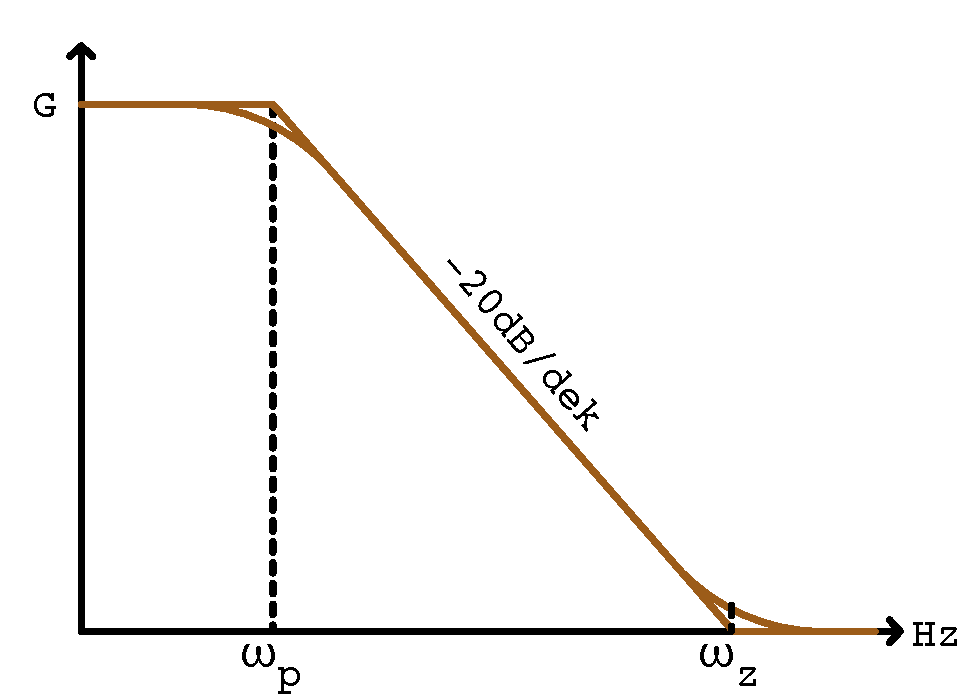
\includegraphics[resolution=300,scale=\circuitSize]{Figure/DesignAfFilter/FoersteordensFilter.pdf}
	\caption{Hældningen for et første ordens lavpasfilter.}
	\label{fig:1OrdensFilter}
\end{figure}
\noindent
%
På \autoref{fig:1OrdensFilter} illustreres hældningen per dekade for et første ordens lavpasfilter med tilhørende pol, $\omega_p$ og nulpunkt, $\omega_z$. Overføringsfunktionen for et første ordens lavpasfilter, er som følger:
%
\begin{equation}
	H(s) = \frac{G*\left(1+\frac{s}{\omega_z}\right)}{\left(1+\frac{s}{\omega_p}\right)}
\end{equation}  
%
$G$ angiver forstærkningen. For at få en hældning på -20dB/dek ved et første ordens filter gælder følgende forhold mellem pol- og nulpunkt:
%
\begin{equation}
	\frac{\omega_z}{\omega_p} > 10
\end{equation} 
%
Hvorimod hvis der skal forstærkes med mindre end -20dB/dek gælder det at:
%
\begin{equation}
	\frac{\omega_z}{\omega_p} < 10
\end{equation}
%
Da filtre generelt angiver en forstærkning eller dæmpning per dekade, er det nødvendigt at beregne hvor meget en forstærkning på 2.62dB mellem 20Hz og 1000Hz vil svarer til per dekade, først beregnes dekaden:
%
\begin{equation}
	log_{10}\left(\frac{1000Hz}{20Hz}\right) = 1.699dek
\end{equation}
%
Så kan forstærkningen per dekade beregnes: 
%
\begin{equation}
	\frac{2.62dB}{1.699dek} = 1.5421dB/dek
\end{equation}
%
Da der både udvikles filtre der forstærker og dæmper vil forstærkningen være $\pm$1.5421dB/dek. 

Ved lave hældninger over et større frekvens område, kan det blive nødvendigt at tilføje flere pol/nulpunkt par. I følgende afsnit vil det blive undersøgt hvor mange af disse par, der er nødvendige for at få den korrekte forstærkning. 
\subsection{Antal pol/nulpunkt par}
\label{AntalPol_Nulpunktpar}
%
Et pol/nulpunkt par angiver at, der er et RC-led i tilbagekoblingen. Et RC-led består af en modstand i serie med en kondensator, hvor modstanden sørger for at forstærkningen er korrekt og kondensatoren sørger for knækfrekvensen, hvor hældningen begynder at falde.
Inden det afgøres hvor mange pol/nulpunkt par der skal anvendes, er det nødvendigt at omregne forstærkningen i dB, $G_{0(dB)}$, til en råforstærkning $G_0$:
%
\begin{equation}
	20*log_{10}(G_0) = G_{0(dB)} = 2.62dB
\end{equation}
%
Derfra isoleres $G_0$:
%
\begin{equation}
	G_0 = 10^{\frac{G_{0(dB)}}{20}} = 10^{\frac{2.62dB}{20}} = 1.3521
	\label{equ:Gain}
\end{equation}
%
For at få en indikation af hvor mange pol/nulpunkt par, svarende til antallet af RC-led, der skal anvendes udarbejdes \autoref{fig:1-8RC-ledIkkeJusteretC}.
%
\begin{figure}[H]
	\centering
	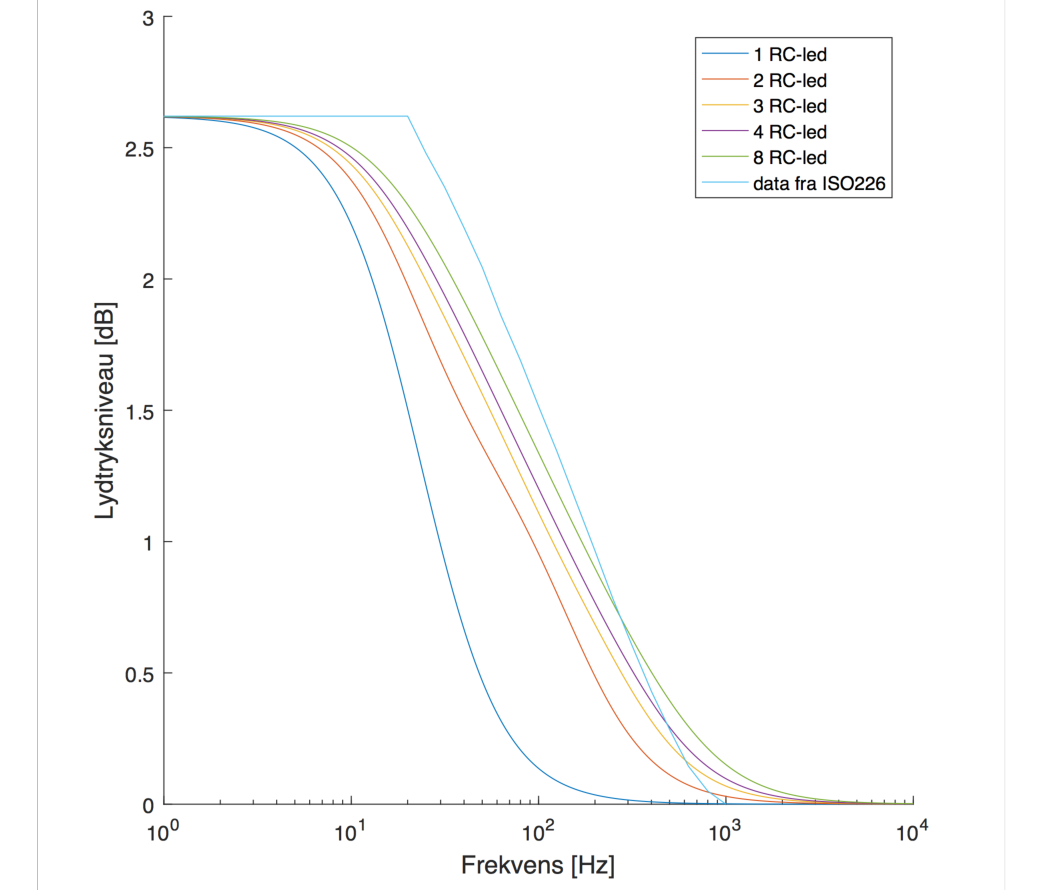
\includegraphics[resolution=300,width=\textwidth]{Figure/DesignAfFilter/1,2,3,4,8RC-ledGain2,62SHORT.pdf}
	\caption{Hældning per dekade for henholdsvis 1, 2, 3, 4 og 8 RC-led, hvor den logaritmiske x-akse angiver frekvens i hertz og den lineære y-akse angiver lydtryksniveau i dB.}
	\label{fig:1-8RC-ledIkkeJusteretC}
\end{figure}
\noindent
%
Kurven for $data fra ISO226$, på \autoref{fig:1-8RC-ledIkkeJusteretC}, repræsenterer resultatet af den teoretisk bedste overføringsfunktion, hvor knækket er ved præcis 20Hz, hvorfor der intet indrulningsforløb er, og hældningen er lineær mellem 20Hz og 1000Hz. RC-ledende er beregnet ud fra en forstærkning på 2.62dB, og samtlige udregninger er vedlagt i \autoref{app:Beregninger af RC-led}. Ydermere er polen valgt ved 20Hz, hvorfra kondensatorværdien udregnes:
%
\begin{equation}
	\omega_z = \frac{1}{R*C}		
\end{equation}  
%
Hvor nulpunktet $\omega_z$ er:
%
\begin{equation}
	\omega_z = 2*\pi*f 
\end{equation}
%
Isoleres kondensatoren, $C$, fåes følgende udtryk:
%
\begin{equation}
	C = \frac{1}{R*\omega_z} = \frac{1}{R*2*\pi*f}
\end{equation} 
%
Beregningerne for de RC-led der repræsenteres på \autoref{fig:1-8RC-ledIkkeJusteretC} fremgår i \autoref{app:Beregninger af RC-led}, og vil derfor ikke blive inkluderet her. Målet er at vælge det antal pol/nulpunkt par, antal RC-led, som sikre linearitet mellem 20Hz og 1000Hz, under den forudsætning at ved 20Hz skal der være en forstærkning på 2.62dB og ved 1000Hz skal der være en forstærkning på 0dB. På baggrund af det fravælges et RC-led, da hældningen er for stejl og der er ingen mulighed for at ændre på hældningen, da pol/nulpunkt parret kun har en effekt på x-aksen. 

Endvidere fravælges det at arbejde med to RC-led, da det ikke opnår en ren linearitet mellem 20Hz og 1000Hz, som det fremgår på \autoref{fig:1-8RC-ledIkkeJusteretC} er der et mindre knæk på kurven. Derimod hvis der arbejdes med tre RC-led opnåes et næsten fuldkomment lineært forløb mellem 20Hz og 1000Hz, jævnfør \autoref{fig:1-8RC-ledIkkeJusteretC}, dog forekommer der både et indrulnings- og udrulningsforløb, som skal justeres for at målet kan opfyldes. Da målet om linearitet mellem 20Hz og 1000Hz ikke forbedres ved at vælge fire eller otte RC-led, fravælges disse og der arbejdes derfor kun med tre RC-led.

På baggrund af det bliver hvert af de fire fraktal ordens filte, som skal sørger for at forstærkningen af de lave frekvenser foregår i overensstemmelse med forstærkningen fremsat i \autoref{tab:ForstaerkningTilDeSyvFiltre}, designet med  tre pol/nulpunkt par, og dermed tre RC-led.
%
\newpage
\noindent
% 
\subsection{Dimensionering af filter med 2.62dBs forstærkning}
\label{DimensioneringAfFilter2.62}
%
Da der arbejdes med tre RC-led er det nødvendigt dele den samlede forstærkning i dB, i tre lige store dele, som illustreret på \autoref{fig:GainOpdeling}.
%
\begin{figure}[H]
	\centering
	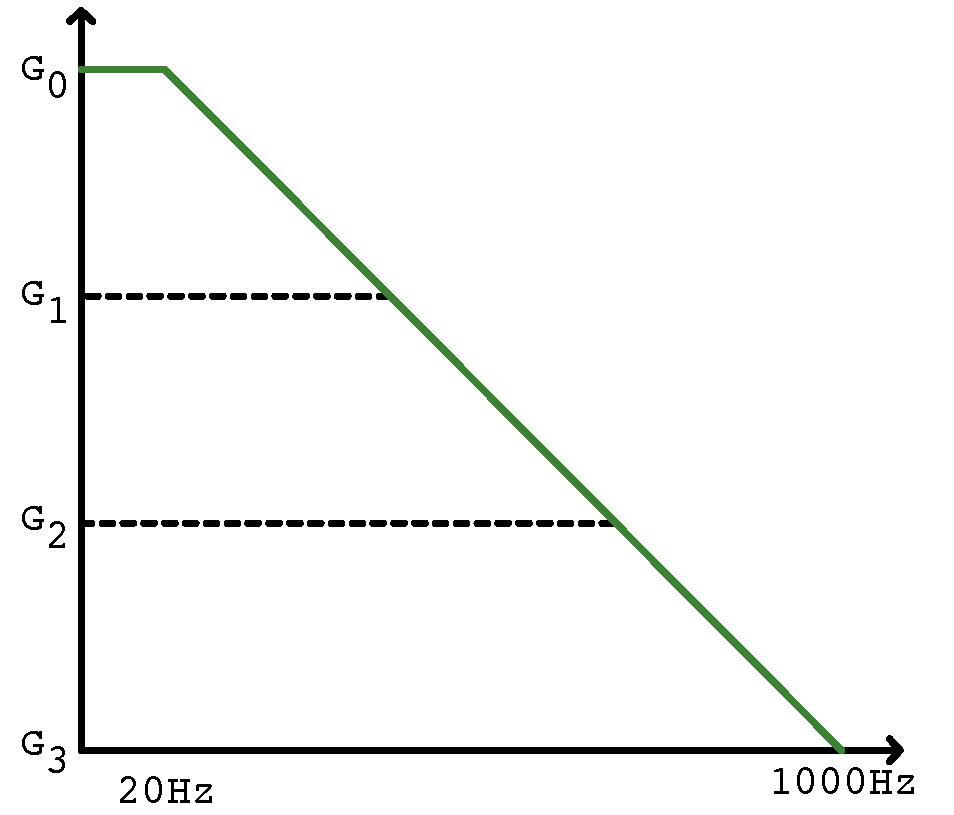
\includegraphics[resolution=300,scale=\circuitSize]{Figure/DesignAfFilter/GainOpdeling.pdf}
	\caption{Illustration af forstærkningsopdelingen, hvor x-aksen angiver frekvens og y-aksen angiver forstærkningen.}
	\label{fig:GainOpdeling}
\end{figure}
\noindent
%
Det første forstærkningstrin skal sørge for at ved 20Hz er der en forstærkning på 2.62dB og det sidste forstærkningstrin sørger for at ved 1000Hz er der en forstærkning på 0dB. De to trin derimellem sørger for at forstærkningen foregår lineært. For at få denne opdeling af forstærkning vil det først blive regnet ud i forhold til forstærkningen i dB, og derefter i forhold til råforstærkning: 
%
\begin{equation}
	G_{0(dB)} = \frac{3}{3}*2.62dB = 2.62dB
\end{equation} 
%
\begin{equation}
	G_{1(dB)} = \frac{2}{3}*2.62dB = 1.7467dB
\end{equation}
%
\begin{equation}
	G_{2(dB)} = \frac{1}{3}*2.62dB = 0.8733dB
\end{equation}
%
\begin{equation}
	G_{3(dB)} = \frac{0}{3}*2.62dB = 0dB
\end{equation}
%
Baseret på \autoref{equ:Gain} omregnes forstærkningerne i dB til den tilsvarende råforstærkning.
%
\begin{equation}
	G_0 = 10^\frac{2.62dB}{20} = 1.3521
\end{equation}
%
\begin{equation}
	G_1 = 10^\frac{1.7467dB}{20} = 1.2227
\end{equation}
%
\begin{equation}
	G_2 = 10^\frac{0.8733dB}{20} = 1.1058
\end{equation}
%
\begin{equation}
	G_3 = 10^\frac{0}{20} = 1
\end{equation}
%
For at beregne hvor store modstandende og kondensatorerne skal være i de tre tilbagekoblede RC-led, er det nødvendigt at tage et led ad gangen. 
%
\begin{figure}[H]
	\centering
	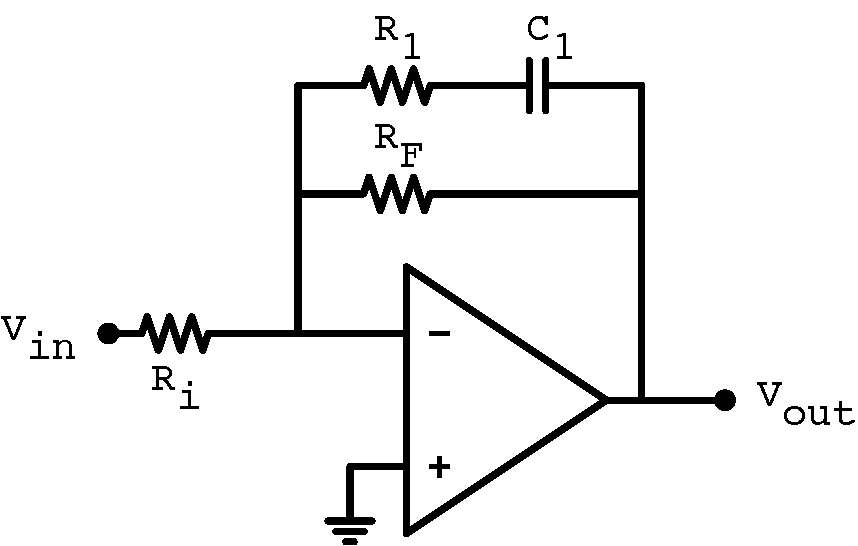
\includegraphics[resolution=300,scale=\circuitSize]{Figure/DesignAfFilter/FilterWith1.pdf}
	\caption{Kredsløbsdiagram for et lavpasfilter med et RC-led.}
	\label{fig:ELdiagramForFilter}
\end{figure}
\noindent
%
Modstanden $R_i$ vælges til 10k$\Omega$, og gør sig gældende for de efterfølgende beregninger af de tre RC-led. Den første overføringsfunktion relaterer sig til at beregne $G_0$ baseret på forholdet mellem $R_i$ og $R_F$:
%
\begin{equation}
	G_0 = -\frac{R_F}{R_i} \Rightarrow R_F = G_0*R_i
	\label{equ:Tilbagekoblingsmodstand}
\end{equation}
%
\begin{equation}
	R_F =  1.3521*10k\Omega = 13.521k\Omega
\end{equation}
%
Med udgangspunkt i et RC-led, som illustreret på \autoref{fig:ELdiagramForFilter} udledes følgende overføringsfunktion:
%
\begin{equation}
	\frac{V_{out}}{V_{in}} = -\frac{R_F||\left(R_1+\frac{1}{s*C_1}\right)}{R_i}
\end{equation}
%
\begin{equation}
	= - \frac{\frac{R_F*\left(R_1+\frac{1}{s*C_1}\right)}{R_F+\left(R_1+\frac{1}{s*C_1}\right)}}{R_i}
\end{equation}
%
\begin{equation}
	= - \frac{R_F*\left(R_1+\frac{1}{s*C_1}\right)}{R_i*\left(R_F+\left(R_1+\frac{1}{s*C_1}\right)\right)}
\end{equation}
%
Udtrykket reduceres ved at multiplicere $s*C_1$ i tæller og nævner:
%
\begin{equation}
	= - \frac{R_F*\left(s*C_1*R_1+1\right)}{R_i*\left(s*C_1*R_F+\left(s*C_1*R_1+1\right)\right)}
\end{equation}
%
Så kan $-R_F$ og $R_i$ trækkes ud:
%
\begin{equation}
	= -\frac{R_F}{R_i}*\frac{s*C_1*R_1+1}{s*C_1*\left(R_F+R_1\right)+1}
\end{equation}
% 
Hvis $C_1$ $\longrightarrow$ $\infty$ vil det resultere i en DC-forstærkning på:
%
\begin{equation}
	\frac{V_{out}}{V_{in}} = -\frac{R_F}{R_i}*1
\end{equation}
%
Hvis det ikke er tilfældet, og $C_1$ ikke går mod $\infty$ så vil der være et pol/nulpunkt par, hvor nulpunktet udledes ved:
%
\begin{equation}
	\omega_z = \frac{1}{R*C} 
\end{equation}
%
\begin{equation}
	 s*C_1*R_1 = \frac{s}{\omega_z}
\end{equation}
%
Og polen ved:
%
\begin{equation}
	\omega_p = \frac{1}{C_1\left(R_F+R_1\right)}
\end{equation}
%
\begin{equation}
	s*C_1\left(R_F+R_1\right) = \frac{s}{\omega_p}
\end{equation}
%
Derfra udledes den endelige overføringsfunktion:
%
\begin{equation}
	\frac{V_{out}}{V_{in}} = -\frac{R_F}{R_i}*\frac{\left(\frac{s}{\omega_z}+1\right)}{\left(\frac{s}{\omega_p}+1\right)}
\end{equation}
%
Hvis $f = \infty$ så bliver impedansen af tilbagekoblingen parallelforbindelsen mellem $R_1||R_F$, hvorfra det fåes:
%
\begin{equation}
	\frac{R_1||R_F}{R_i}
\end{equation}
% 
Herfra er det muligt at beregne modstanden $R_1$ ved at udlede følgende udtryk. Først tilføjes der en modstand $R_F'$, som udgør parallelforbindelse mellem $R_F$ og $R_1$:
%
\begin{equation}
	R_F' = \frac{R_F*R_1}{R_F+R_1}
	\label{equ:R_FMaerke}
\end{equation}
%
$R_F'$ vil svare til $R_F$, illustreret på \autoref{fig:ELdiagramForFilter}, når der regnes med to RC-led. Da tilbagekoblingsmodstanden beregnes ud fra \autoref{equ:Tilbagekoblingsmodstand} er det muligt at anvende samme ligning til at beregne $R_F'$:
%
\begin{equation}
	R_F' = G_1*R_i = 1.2227*10k\Omega = 12.227k\Omega
\end{equation}
%
Da der ikke tages højde for at $R_1$ sidder i serie med $C_1$, isoleres $R_1$ i \autoref{equ:R_FMaerke}:
%
\begin{equation}
	R_1 = \frac{R_F*R_F'}{R_F-R_F'} = \frac{13.521k\Omega*12.227k\Omega}{13.521k\Omega-12.227k\Omega} = 127.826k\Omega
\end{equation}  
%
Overføringsfunktionerne fremsat for et RC-led vil være de samme for både to og tre RC-led, dog med forbehold for at $R_F$ erstattes med $R_F'$ ved to RC-led og $R_F''$ ved tre RC-led, og $R_1$ bliver erstattet med henholdvis $R_2$ og $R_3$. Derudover erstattes $C_1$ med henholdvis $C_2$ og $C_3$. I \autoref{app:Overfoeringsfunktion} fremgår overføringsfunktionerne for henholdvist to og tre RC-led.

De efterfølgende beregninger foretages for to RC-led, hvorfra det er muligt at beregne modstanden $R_2$ ved at udlede følgende udtryk. Først tilføjes der en modstand $R_F''$, som udgør parallelforbindelsen mellem $R_F'$ og $R_2$
%
\begin{equation}
	R_F'' = \frac{R_F'*R_2}{R_F'+R_2}
	\label{equ:R_FMaerke2}
\end{equation}
%
$R_F''$ vil svare til $R_F$, illustreret på \autoref{fig:ELdiagramForFilter}, når der regnes med tre RC-led. Da tilbagekoblingsmodstanden beregnes ud fra \autoref{equ:Tilbagekoblingsmodstand} er det muligt at anvende samme ligning til at beregne $R_F''$:
%
\begin{equation}
	R_F'' = G_2*R_i = 1.1058*10k\Omega = 11.058k\Omega	
\end{equation}
%
Da der ikke tages højde for at $R_2$ sidder i serie med $C_2$, isoleres $R_2$ i \autoref{equ:R_FMaerke2}:
%
\begin{equation}
	R_2 = \frac{R_F'*R_F''}{R_F'-R_F''} = \frac{12.227k\Omega*11.058k\Omega}{12.227k\Omega-11.058k\Omega} = 115.598k\Omega
\end{equation}  
%
De efterfølgende beregninger foretages for tre RC-led, hvorfra det er muligt at beregne modstanden $R_3$ ved at udlede følgende udtryk. Først tilføjes der en modstand $R_F'''$, som udgør parallelforbindelsen mellem $R_F''$ og $R_3$
%
\begin{equation}
	R_F''' = \frac{R_F''*R_3}{R_F''+R_3}
	\label{equ:R_FMaerke3}
\end{equation}
%
$R_F'''$ vil svare til $R_F$, illustreret på \autoref{fig:ELdiagramForFilter}, når der regnes med tre RC-led. Da tilbagekoblingsmodstanden beregnes ud fra \autoref{equ:Tilbagekoblingsmodstand} er det muligt at anvende samme ligning til at beregne $R_F'''$:
%
\begin{equation}
	R_F''' = G_3*R_i = 1*10k\Omega = 10k\Omega	
\end{equation}
%
Da der ikke tages højde for at $R_3$ sidder i serie med $C_3$, isoleres $R_3$ i \autoref{equ:R_FMaerke3}:
%
\begin{equation}
	R_3 = \frac{R_F''*R_F'''}{R_F''-R_F'''} = \frac{11.058k\Omega*10k\Omega}{11.058k\Omega-10k\Omega} = 104.541k\Omega
\end{equation}  
%
Nu er det muligt at udregne de tre knækfrekvenser, hvorfra kondensatorværdierne skal beregnes, hvilket gøres ved at opdele den logaritmiske x-akse i tre lige stor dele, ligesom tilfældet med forstærkningen, jævnfør \autoref{fig:GainOpdeling}. Følgende udtryk anvendes til at opdele aksen i tre lige store dele:
%
\begin{equation}
	f_{logstep} = \frac{1}{3}*log_{10}\left(\frac{f_{high}}{f_{low}}\right)
\end{equation}
%
$f_{high}$ og $f_{low}$ angiver henholdsvis den største og mindste frekvens, som opdelingen skal foretages inden for, derfor er: $f_{high}$ 1000Hz og $f_{low}$ 20Hz.
%
\begin{equation}
	f_{logstep} = \frac{1}{3}*log_{10}\left(\frac{1000Hz}{20Hz}\right) = 0.566
\end{equation}
%
Her fra kan polerne for de tre RC-led udledes:
%
\begin{equation}
	p_1 = 20Hz
\end{equation}
%
\begin{equation}
	p_2 = p_1*10^{1*f_{logstep}} = 73.681Hz
\end{equation}
%
\begin{equation}
	p_3 = p_1*10^{2*f_{logstep}} = 271.442Hz
\end{equation}
%
\begin{equation}
	p_4 = p_1*10^{3*f_{logstep}} = 1000Hz
\end{equation}
%
Baseret på de tre poler er det muligt at beregne de tre kondensatorværdier:
%
\begin{equation}
	C_1 = \frac{1}{(R_1+R_F)*2*\pi*p_1} 
\end{equation}
%
\begin{equation}
	C_1 = \frac{1}{(127.826k\Omega+13.521k\Omega)*2*\pi*20Hz} = 56.3nF
\end{equation}
%
\begin{equation}
	C_2 = \frac{1}{(R_2+R_F')*2*\pi*p_2}
\end{equation}
%
\begin{equation}
	 C_2 = \frac{1}{(115.598k\Omega+12.227k\Omega)*2*\pi*73.681Hz} = 16.889nF
\end{equation}
%
\begin{equation}
	C_3 = \frac{1}{(R_3+R_F'')*2*\pi*p_3} 
\end{equation}
%
\begin{equation}
	C_3 = \frac{1}{(104.541k\Omega+11.058k\Omega)*2*\pi*271.442Hz} = 5.072nF
\end{equation}
%
Når både modstandende og kondensatorværdierne simuleres, resulterer det i  kurven for 20Hz på \autoref{fig:JusteretPol}. \\[5mm]
%
Som nævnt tidligere er det muligt, ved at ændre på forholdet mellem pol og nulpunktet, at forskyde hældningen på x-aksen. Det gøres for at forskyde indrulnignsforløbet, så det er overstået før 20Hz, da forstærkningen ved 20Hz skal være 2.62dB. Ved hjælp af simuleringer estimeres det at den første pol bør være ved 55Hz, hvilket resulterer i nye udregning af de tre kondensatorværdier:
%
\begin{equation}
	p_1 = 55Hz
\end{equation}
%
\begin{equation}
	p_2 = p_1*10^{1*f_{logstep}} = 144.624Hz
\end{equation}
%
\begin{equation}
	p_3 = p_1*10^{2*f_{logstep}} = 380.295Hz
\end{equation}
%
\begin{equation}
	p_4 = p_1*10^{3*f_{logstep}} = 1000Hz
\end{equation}
%
Baseret på de tre poler er det muligt at beregne de tre kondensatorværdier:
%
\begin{equation}
	C_1 = \frac{1}{(R_1+R_F)*2*\pi*p_1} 
\end{equation}
%
\begin{equation}
	C_1 = \frac{1}{(127.826k\Omega+13.521k\Omega)*2*\pi*55Hz} = 20.473nF
\end{equation}
%
\begin{equation}
	C_2 = \frac{1}{(R_2+R_F')*2*\pi*p_2} 
\end{equation}
%
\begin{equation}
	C_2 = \frac{1}{(115.598k\Omega+12.227k\Omega)*2*\pi*144.624Hz} = 8.609nF
\end{equation}
\begin{equation}
	C_3 = \frac{1}{(R_3+R_F'')*2*\pi*p_3} 
\end{equation}
%
\begin{equation}
	C_3 = \frac{1}{(104.541k\Omega+11.058k\Omega)*2*\pi*380.295Hz} = 3.62nF
\end{equation}
%
Når disse værdier tilsvarende simuleres, resulterer det i kurven for 55Hz på \autoref{fig:JusteretPol}, som i højere grad stemmer over ens med kurven for ISO226 på samme \autoref{fig:JusteretPol}.
%
\begin{figure}[H]
	\centering
	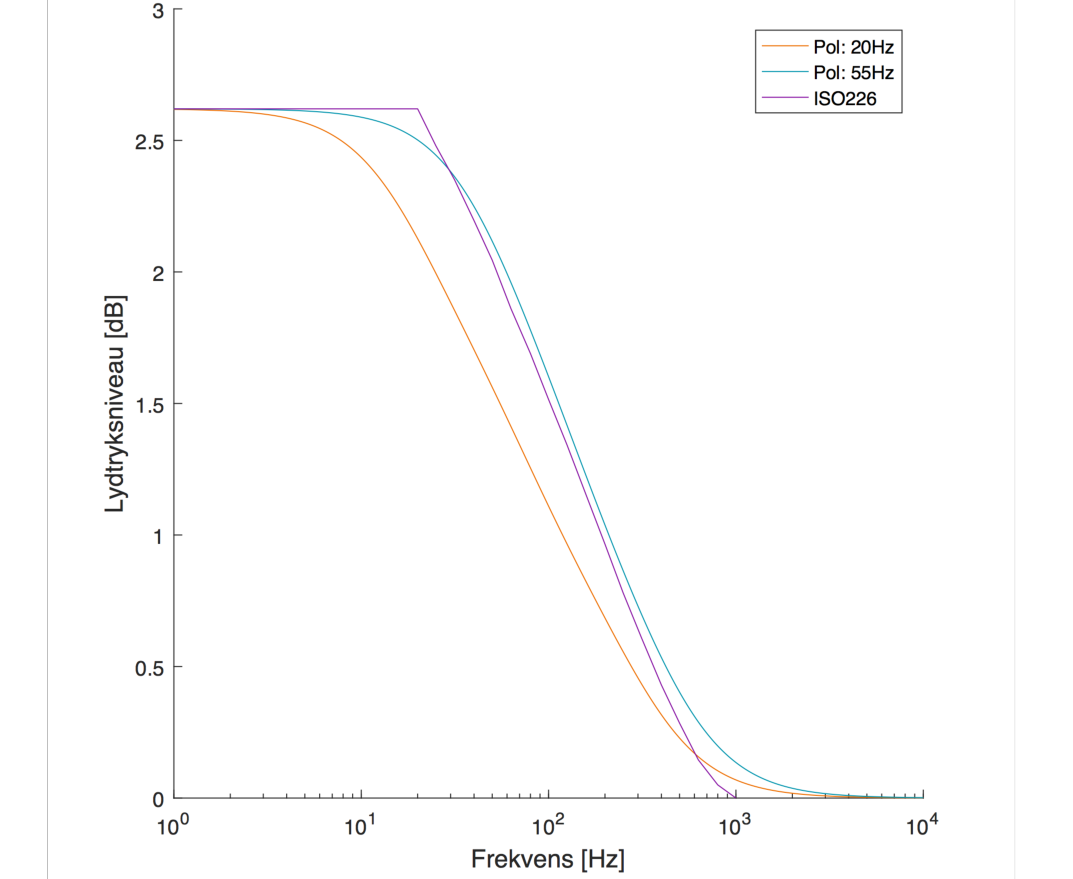
\includegraphics[resolution=300,width=\textwidth]{Figure/DesignAfFilter/JusteretPolSHORT.pdf}
	\caption{Justering af modstands- og kondensatorværdier for tre RC-led i forhold til ISO226.}
	\label{fig:JusteretPol}
\end{figure}
\noindent
%
Designet af det filter der skal forstærke 20Hz med 2.62dB, bliver udviklet i henhold til de foregående udregninger, som resulterer i kurven for 55Hz på \autoref{fig:JusteretPol}. Dertil bliver de restende filtre udviklet i henhold til de beregninger der foretages i de efterfølgende afsnits vedrørende dimensionering.
%
\begin{figure}[H]
	\centering
	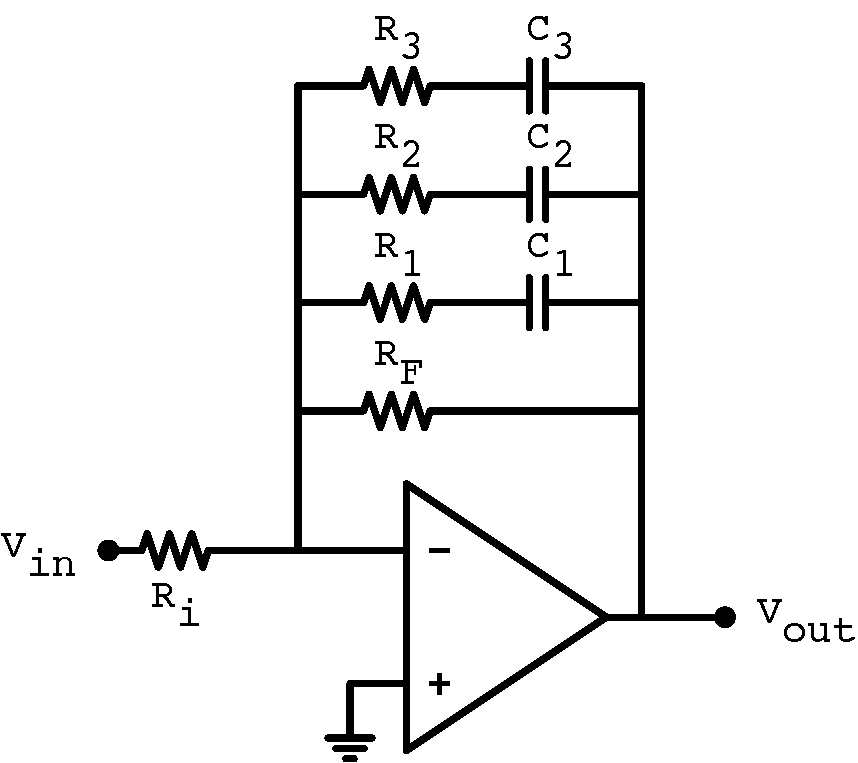
\includegraphics[resolution=300,scale=\circuitSize]{Figure/DesignAfFilter/FilterWith3.pdf}
	\caption{Kredsløbsdiagram for de fire filtre der skal forstærke de lave frekvenser.}
	\label{fig:ElDiagramFor3RC}
\end{figure}
\noindent
%
\newpage
\noindent
%
Uanset hvilken forstærkning modstandende og kondensatorværdierne bliver udregnet fra, så er kredsløbsdiagrammet på \autoref{fig:ElDiagramFor3RC} gældende for alle.
%

\subsection{Dimensionering af filter med 5.24dB's forstærkning}
\label{DimensioneringAfFilter5.24}
%
Fremgangsmåden for dimensionering af det filter der skal forstærke med 5.24dB er præcis den samme, som ved \fullref{DimensioneringAfFilter2.62}, dog tages der udgangspunkt i en anden forstærkning, de fuldkomne beregninger er vedlagt i \autoref{app:3RCledGain5.24}. For ikke at skulle gennemgå alle beregningerne igen, listes værdierne i de efterfølgende tabeller
%
\begin{table}[H]
\centering
\begin{tabular}{|r|r|r|r|r|r|r|r|}
\hline
\multicolumn{1}{|l|}{$G_{0dB}$} & \multicolumn{1}{l|}{$G_{1dB}$} & \multicolumn{1}{l|}{$G_{2dB}$} & \multicolumn{1}{l|}{$G_{3dB}$} & \multicolumn{1}{l|}{$G_0$} & \multicolumn{1}{l|}{$G_1$} & \multicolumn{1}{l|}{$G_2$} & \multicolumn{1}{l|}{$G_3$} \\ \hline
5.24dB & 3.493dB & 1.747dB & 0dB & 1.828 & 1.4951 & 1.2227 & 1\\ \hline
\end{tabular}
\caption{Oversigt over forstærkningen i dB og råforstærkningen, ved opdeling illustreret på \autoref{fig:GainOpdeling}.}
\label{tab:DimensioneringAf5.24Gain}
\end{table}
\noindent
%
%
\begin{table}[H]
\centering
\begin{tabular}{|r|r|r|r|r|r|r|}
\hline
\multicolumn{1}{|l|}{$R_F$} & \multicolumn{1}{l|}{$R_F'$} & \multicolumn{1}{l|}{$R_F''$} & \multicolumn{1}{l|}{$R_F'''$} & \multicolumn{1}{l|}{$R_1$} & \multicolumn{1}{l|}{$R_2$} & \multicolumn{1}{l|}{$R_3$} \\ \hline
18.281k$\Omega$ & 14.951k$\Omega$ & 12.227k$\Omega$ & 10k$\Omega$ & 82.074k$\Omega$ & 67.123k$\Omega$ & 54.896$k\Omega$\\ \hline
\end{tabular}
\caption{Oversigt over tilbagekoblingsmodstandene og de tre andre modstande.}
\label{tab:DimensioneringAf5.24Modstand}
\end{table}
\noindent
%

%
\begin{table}[H]
\centering
\begin{tabular}{|r|r|r|r|r|r|r|}
\hline
\multicolumn{1}{|l|}{$p_1$} & \multicolumn{1}{l|}{$p_2$} & \multicolumn{1}{l|}{$p_3$} & \multicolumn{1}{l|}{$p_4$} & \multicolumn{1}{l|}{$C_1$} & \multicolumn{1}{l|}{$C_2$} & \multicolumn{1}{l|}{$C_3$} \\ \hline
55Hz & 144.624Hz & 380.295Hz & 1000Hz & 28.835nF & 13.408nF & 6.235nF \\ \hline
\end{tabular}
\caption{Oversigt over knækfrevkserne for polerne og kondensatorværdierne.}
\label{tab:DimensioneringAf5.24polC}
\end{table}
\noindent
%

\subsection{Dimensionering af filter med 10.48dB's forstærkning}
\label{DimensioneringAfFilter10.48}
% 
Fremgangsmåden for dimensionering af det filter der skal forstærke med 10.48dB er præcis den samme, som ved \fullref{DimensioneringAfFilter2.62}, dog tages der udgangspunkt i en anden forstærkning, de fuldkomne beregninger er vedlagt i \autoref{app:3RCledGain10.48}. For ikke at skulle gennemgå alle beregningerne igen, listes værdierne i de efterfølgende tabeller
%
\begin{table}[H]
\centering
\begin{tabular}{|r|r|r|r|r|r|r|r|}
\hline
\multicolumn{1}{|l|}{$G_{0dB}$} & \multicolumn{1}{l|}{$G_{1dB}$} & \multicolumn{1}{l|}{$G_{2dB}$} & \multicolumn{1}{l|}{$G_{3dB}$} & \multicolumn{1}{l|}{$G_0$} & \multicolumn{1}{l|}{$G_1$} & \multicolumn{1}{l|}{$G_2$} & \multicolumn{1}{l|}{$G_3$} \\ \hline
10.48dB & 6.987dB & 3.493dB & 0dB & 3.342 & 2.2353 & 1.4951 & 1\\ \hline
\end{tabular}
\caption{Oversigt over forstærkningen i dB og råforstærkningen, ved opdeling illustreret på \autoref{fig:GainOpdeling}.}
\label{tab:DimensioneringAf10.48Gain}
\end{table}
\noindent
%
%
\begin{table}[H]
\centering
\begin{tabular}{|r|r|r|r|r|r|r|}
\hline
\multicolumn{1}{|l|}{$R_F$} & \multicolumn{1}{l|}{$R_F'$} & \multicolumn{1}{l|}{$R_F''$} & \multicolumn{1}{l|}{$R_F'''$} & \multicolumn{1}{l|}{$R_1$} & \multicolumn{1}{l|}{$R_2$} & \multicolumn{1}{l|}{$R_3$} \\ \hline
33.42k$\Omega$ & 22.353k$\Omega$ & 14.951k$\Omega$ & 10k$\Omega$ & 67.502k$\Omega$ & 45.149k$\Omega$ & 30.198k$\Omega$\\ \hline
\end{tabular}
\caption{Oversigt over tilbagekoblingsmodstandene og de tre andre modstande.}
\label{tab:DimensioneringAf10.48Modstand}
\end{table}
\noindent
%
%
\begin{table}[H]
\centering
\begin{tabular}{|r|r|r|r|r|r|r|}
\hline
\multicolumn{1}{|l|}{$p_1$} & \multicolumn{1}{l|}{$p_2$} & \multicolumn{1}{l|}{$p_3$} & \multicolumn{1}{l|}{$p_4$} & \multicolumn{1}{l|}{$C_1$} & \multicolumn{1}{l|}{$C_2$} & \multicolumn{1}{l|}{$C_3$} \\ \hline
55Hz & 144.624Hz & 380.295Hz & 1000Hz & 28.673nF & 16.303nF & 9.269nF \\ \hline
\end{tabular}
\caption{Oversigt over knækfrevkserne for polerne og kondensatorværdierne.}
\label{tab:DimensioneringAf10.48polC}
\end{table}
\noindent
%
%
\subsection{Dimensionering af filter med 20.96dB's forstærkning}
\label{DimensioneringAfFilter20.96}
%
Fremgangsmåden for dimensionering af det filter der skal forstærke med 20.96dB er præcis den samme, som ved \fullref{DimensioneringAfFilter2.62}, dog tages der udgangspunkt i en anden forstærkning, de fuldkomne beregninger er vedlagt i \autoref{app:3RCledGain20.96}. For ikke at skulle gennemgå alle beregningerne igen, listes værdierne i de efterfølgende tabeller
%
\begin{table}[H]
\centering
\begin{tabular}{|r|r|r|r|r|r|r|r|}
\hline
\multicolumn{1}{|l|}{$G_{0dB}$} & \multicolumn{1}{l|}{$G_{1dB}$} & \multicolumn{1}{l|}{$G_{2dB}$} & \multicolumn{1}{l|}{$G_{3dB}$} & \multicolumn{1}{l|}{$G_0$} & \multicolumn{1}{l|}{$G_1$} & \multicolumn{1}{l|}{$G_2$} & \multicolumn{1}{l|}{$G_3$} \\ \hline
20.96dB & 13.973dB & 6.987dB & 0dB & 11.169 & 4.9965 & 2.2353 & 1\\ \hline
\end{tabular}
\caption{Oversigt over forstærkningen i dB og råforstærkningen, ved opdeling illustreret på \autoref{fig:GainOpdeling}.}
\label{tab:DimensioneringAf20.96Gain}
\end{table}
\noindent
%
%
\begin{table}[H]
\centering
\begin{tabular}{|r|r|r|r|r|r|r|}
\hline
\multicolumn{1}{|l|}{$R_F$} & \multicolumn{1}{l|}{$R_F'$} & \multicolumn{1}{l|}{$R_F''$} & \multicolumn{1}{l|}{$R_F'''$} & \multicolumn{1}{l|}{$R_1$} & \multicolumn{1}{l|}{$R_2$} & \multicolumn{1}{l|}{$R_3$} \\ \hline
111.686k$\Omega$ & 49.965k$\Omega$ & 22.353k$\Omega$ & 10k$\Omega$ & 90.413k$\Omega$ & 40.448k$\Omega$ & 18.095k$\Omega$\\ \hline
\end{tabular}
\caption{Oversigt over tilbagekoblingsmodstandene og de tre andre modstande.}
\label{tab:DimensioneringAf20.96Modstand}
\end{table}
\noindent
%
%
\begin{table}[H]
\centering
\begin{tabular}{|r|r|r|r|r|r|r|}
\hline
\multicolumn{1}{|l|}{$p_1$} & \multicolumn{1}{l|}{$p_2$} & \multicolumn{1}{l|}{$p_3$} & \multicolumn{1}{l|}{$p_4$} & \multicolumn{1}{l|}{$C_1$} & \multicolumn{1}{l|}{$C_2$} & \multicolumn{1}{l|}{$C_3$} \\ \hline
55Hz & 144.624Hz & 380.295Hz & 1000Hz & 14.318nF & 12.172nF & 10.347nF \\ \hline
\end{tabular}
\caption{Oversigt over knækfrevkserne for polerne og kondensatorværdierne.}
\label{tab:DimensioneringAf20.96polC}
\end{table}
\noindent
%
\subsection{Filtre der dæmper}
\label{FiltreDerDaemper}
%
De foregående afsnit har alle fokuseret og taget udgangspunkt i de filtre der skal forstærke de lave frekvenser, men da det også skal kunne lade sig gøre, at dæmpe de lave frekvenser, skal der ligeledes udvikles filtre som understøtter dette. Når det angives at et filter skal dæmpe de lave frekvenser, svarer det til, at de lave frekvenser forstærkes med en forstærkning $G<1$. Rent matematisk kan det udtrykkes ved:\\[5mm]   
%
For én gangs forstærkning, forudsætter det at $R_F = R_i$, og kan udtrykkes ved følgende:
%
\begin{equation}
	G = \frac{V_{out}}{V_{in}} = -\frac{R_F}{R_i}
\end{equation}
%
Såfremt at $R_F>R_i$ vil der ske en forstærkning på $>1$, hvis $R_F$ eksempelvist er dobbelt så stor, som $R_i$ vil forstærkningen være:
%
\begin{equation}
	G = \frac{V_{out}}{V_{in}} = -\frac{R_F}{R_i} = -\frac{2k\Omega}{1k\Omega} = -2
\end{equation}
%
Hvorimod hvis $R_F<R_i$ vil der ske en forstærkning på $<1$, så hvis $R_F$ eksempelvist er halvt så stor, som $R_i$ vil forstærkningen være:
%
\begin{equation}
	G = \frac{V_{out}}{V_{in}} = -\frac{R_F}{R_i} = -\frac{1k\Omega}{2k\Omega} = -0.5
\end{equation}
%
Filtrene der er dæmper de lave frekvenser vil derfor, principielt, forstærke de lave frekvenser med en forstærkning på $<1$. Den samme effekt vil opnåes ved at ændre udtrykket for forstærkningen til:
%
\begin{equation}
	G = \frac{V_{out}}{V_{in}} = -\frac{R_i}{R_F}
\end{equation}
%
Det er derfor muligt, at koble tilbagekoblingsmodstanden $R_F$ samt de tre RC-led på den inverterende terminal, og lade $R_i$ udgøre tilbagekoblingen fra $V_{out}$ til $V_-$, hvilket illustreres på \autoref{fig:FilterDerDaemper}. 
%
\begin{figure}[H]
	\centering
	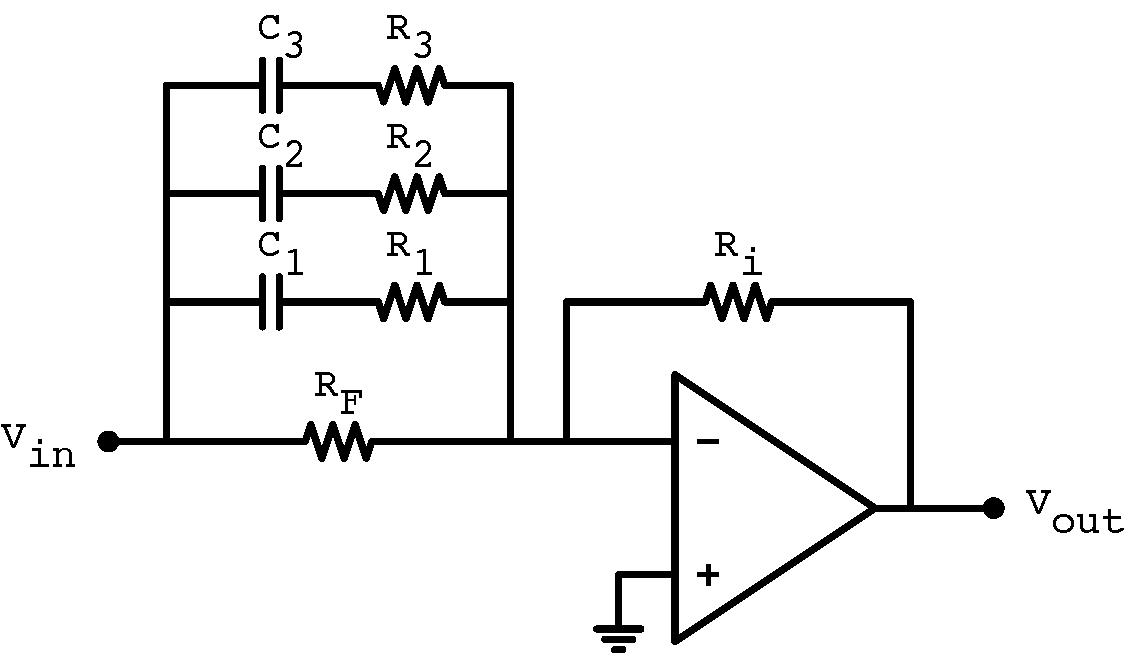
\includegraphics[resolution=300,scale=\circuitSize]{Figure/DesignAfFilter/FilterWithLess3.pdf}
	\caption{Kredsløbsdiagram for de tre filtre der skal dæmpe de lave frekvenser.}
	\label{fig:FilterDerDaemper}
\end{figure}
\noindent
%
Det eneste der ændre sig i forhold til forstærkningen af de lave frekvenser, er fortegnet på forstærkningen i dB, så istedet for at forstærke de lave frekvenser med 2.62dB skal der i disse filtre forstærkes med -2.62dB. Da det er den eneste forskel resulterer det ligeledes i at alle modstands- og kondensatorværdier er ens for de tre RC-led og afhænger kun af om forstærkningen er -2.62dB, -5.24dB eller -10.48dB.
%
\newpage
\noindent
%
\subsection{Opsummering af filtre}
\label{OpsummeringAfFiltre}
%
Baseret på dimensioneringen af de fire filtre der forstærker og de tre der dæmper kan de endelige kurver, som opnår størst linearitet mellem 20Hz og 1000Hz repræsenteres, jævnfør \autoref{fig:EndeligeFiltre}.
%
\begin{figure}[H]
	\centering
	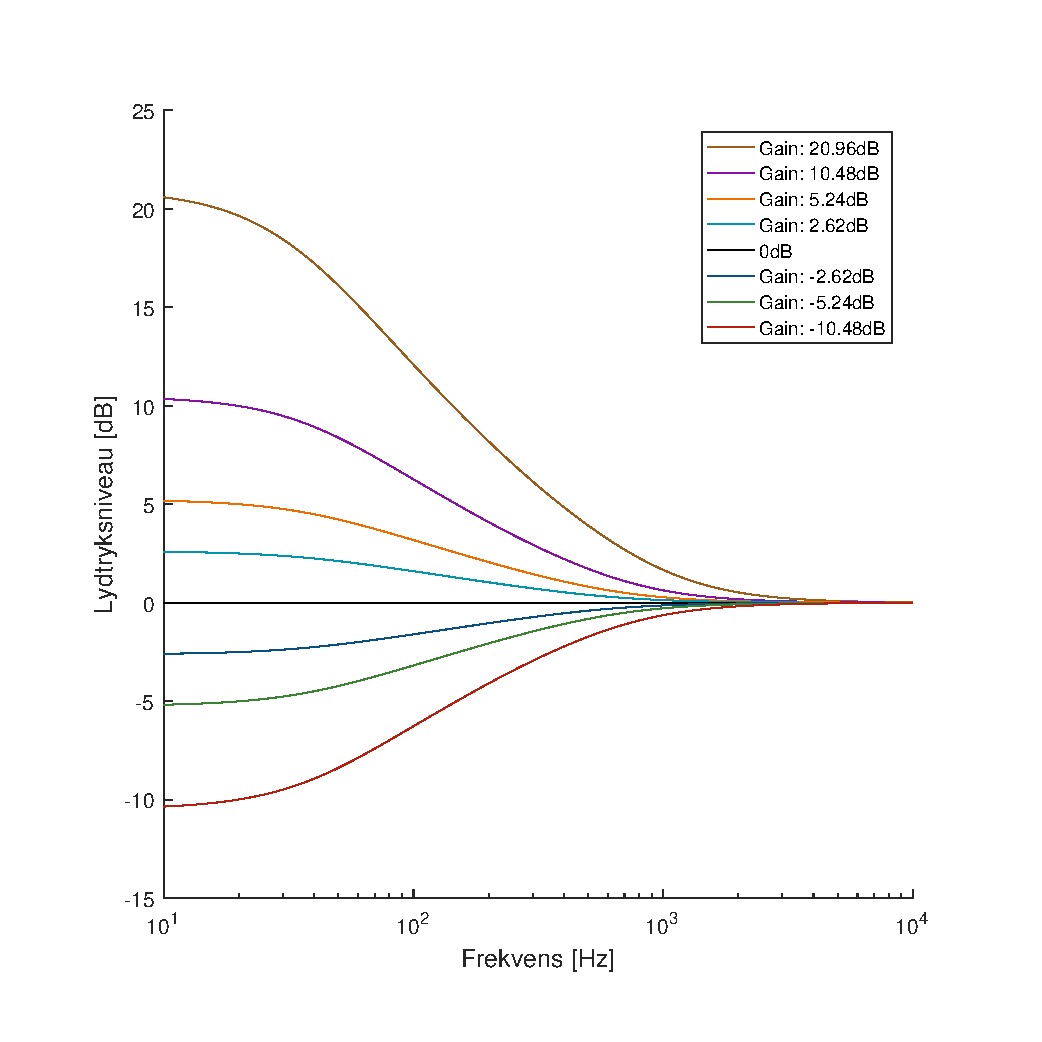
\includegraphics[resolution=300,width=\textwidth]{Figure/DesignAfFilter/EndeligeFiltre.pdf}
	\caption{Hældningerne for de fire filtre der forstærker og de tre der dæmper de lave frekvenser, hvor hver kurve repræsentere én af de syv forstærkninger i dB ved 20Hz.}
	\label{fig:EndeligeFiltre}
\end{figure}
\noindent
%
Sammenholdes kurverne på \autoref{fig:EndeligeFiltre} med resultatet af den teoretisk bedste overføringsfunktion for hver forstærkning, angivet i \autoref{tab:ForstaerkningTilDeSyvFiltre}, hvor knækket er ved præcist 20Hz, hvorfor der intet indrulningsforløb fremgår, og hældningen er lineær mellem 20Hz og 1000Hz. Data til \autoref{fig:EndeligeFiltre} forefindes i vedlagte mappe, som er navngivet: \textit{SupplerendeMateriale}
%
\begin{figure}[H]
	\centering
	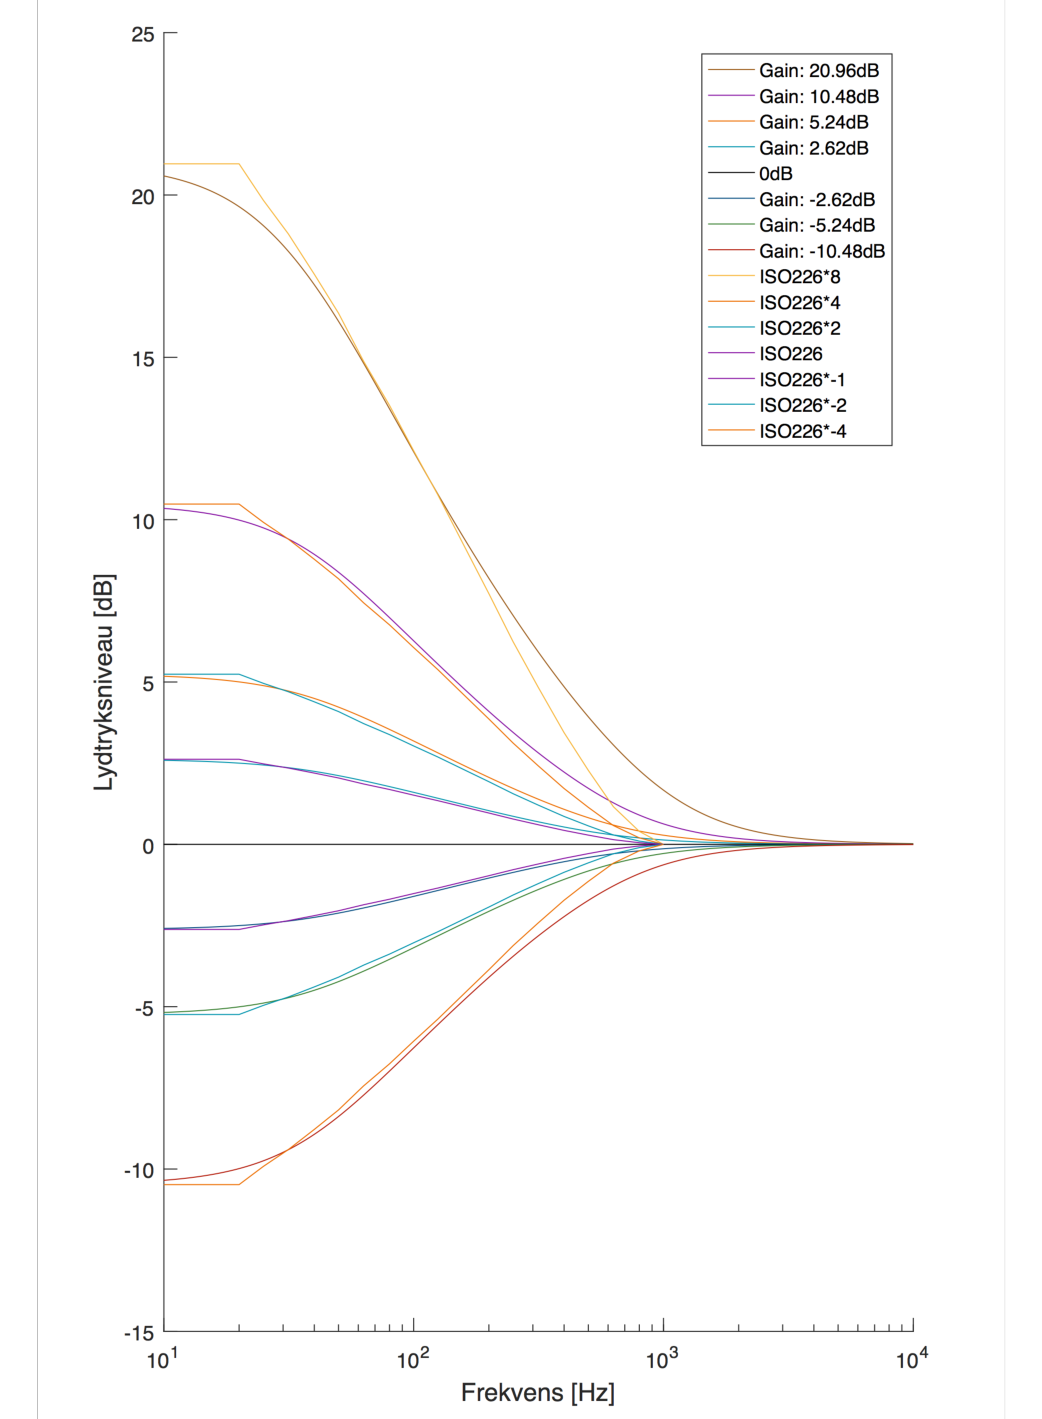
\includegraphics[resolution=300,width=\textwidth]{Figure/DesignAfFilter/EndeligeFiltreMedReferenceSHORT.pdf}
	\caption{Repræsentation af hældningerne for hvert filter sammenlignet med resultatet af den tilsvarende teoretiske bedste overføringsfunktion, hvor forstærkningen fremgår af \autoref{tab:ForstaerkningTilDeSyvFiltre}}.
	\label{fig:EndeligeFiltreMedReference}
\end{figure}
\noindent
%
På \autoref{fig:EndeligeFiltreMedReference} sammenholdes hældningerne fra hvert filter med resultatet af den tilsvarende teoretiske bedste overføringsfunktion, hvor knækket er ved præcist 20Hz, hvorfor der intet indrulningsforløb er, og hældningen er lineær mellem 20Hz og 1000Hz. Det tyder desværre på at ved en forstærkning på 20.96dB bør der foretages nogle justeringer. Disse justeringer kunne være at vælge en mindre pol $(<55Hz)$, for på den måde at forskyde kurven på x-aksen, det vil dog resultere i at kondensatorværdierne næsten vil være ens, og dermed kan det overvejes om det vil være en fordel at fjerne et RC-led. Ved at fjerne et RC-led vil det også resultere i en stejlere hældning. Selvom det er muligt at reducere afvigelsen mellem kurven: $Gain: 20.96dB$ og $ISO226*8$, gøres det ikke og det vælges at arbejde videre med $Gain: 20.96dB$, som den er beregnet.  

\subsection{Tilpasning af filtre}
\label{TilpasningAfFilter}
%
De efterfølgende tabeller lister de beregnede og brugte komponentværdier, afhængigt af hvilket filter de tilhører og hvor stor afvigelsen er. Under hver tabel fremgår det tilhørende, færdige, filter.
%
\begin{equation}
	Afvigelse (\%) = \frac{brugt-beregnet}{beregnet}*100\%
\end{equation}
%
\begin{table}[H]
\centering
\begin{tabular}{|c|r|r|r|}
\hline
\multicolumn{1}{|l|}{Komponenter} & \multicolumn{1}{l|}{Beregnet} & \multicolumn{1}{l|}{Brugt} & \multicolumn{1}{l|}{Afvigelse [$\%$]}\\ \hline
$R_i$ & 10k$\Omega$ & 10k$\Omega$ & 0\\ \hline
$R_F$ & 13.521k$\Omega$ & 13.7k$\Omega$ & 1.3239 \\ \hline
$R_1$ & 127.826k$\Omega$ & 127k$\Omega$ & 0.6462\\ \hline
$R_2$ & 115.598k$\Omega$ & 115k$\Omega$ & 0.5173 \\ \hline
$R_3$ & 104.541k$\Omega$ & 105k$\Omega$ & 0.4391 \\ \hline
$C_1$ & 20.473nF & 22nF & 7.4586 \\ \hline
$C_2$ & 8.604nF & 6.8nF & -20.967 \\ \hline
$C_3$ & 3.62nF & 3.5nF & -3.3149 \\ \hline
\end{tabular}
\caption{Komponentværdier for de filtre der forstærker $\pm$2.62dB.}
\label{tab:TilpasningAfFiltre2.62}
\end{table}
%
\begin{figure}[H]
	\centering
	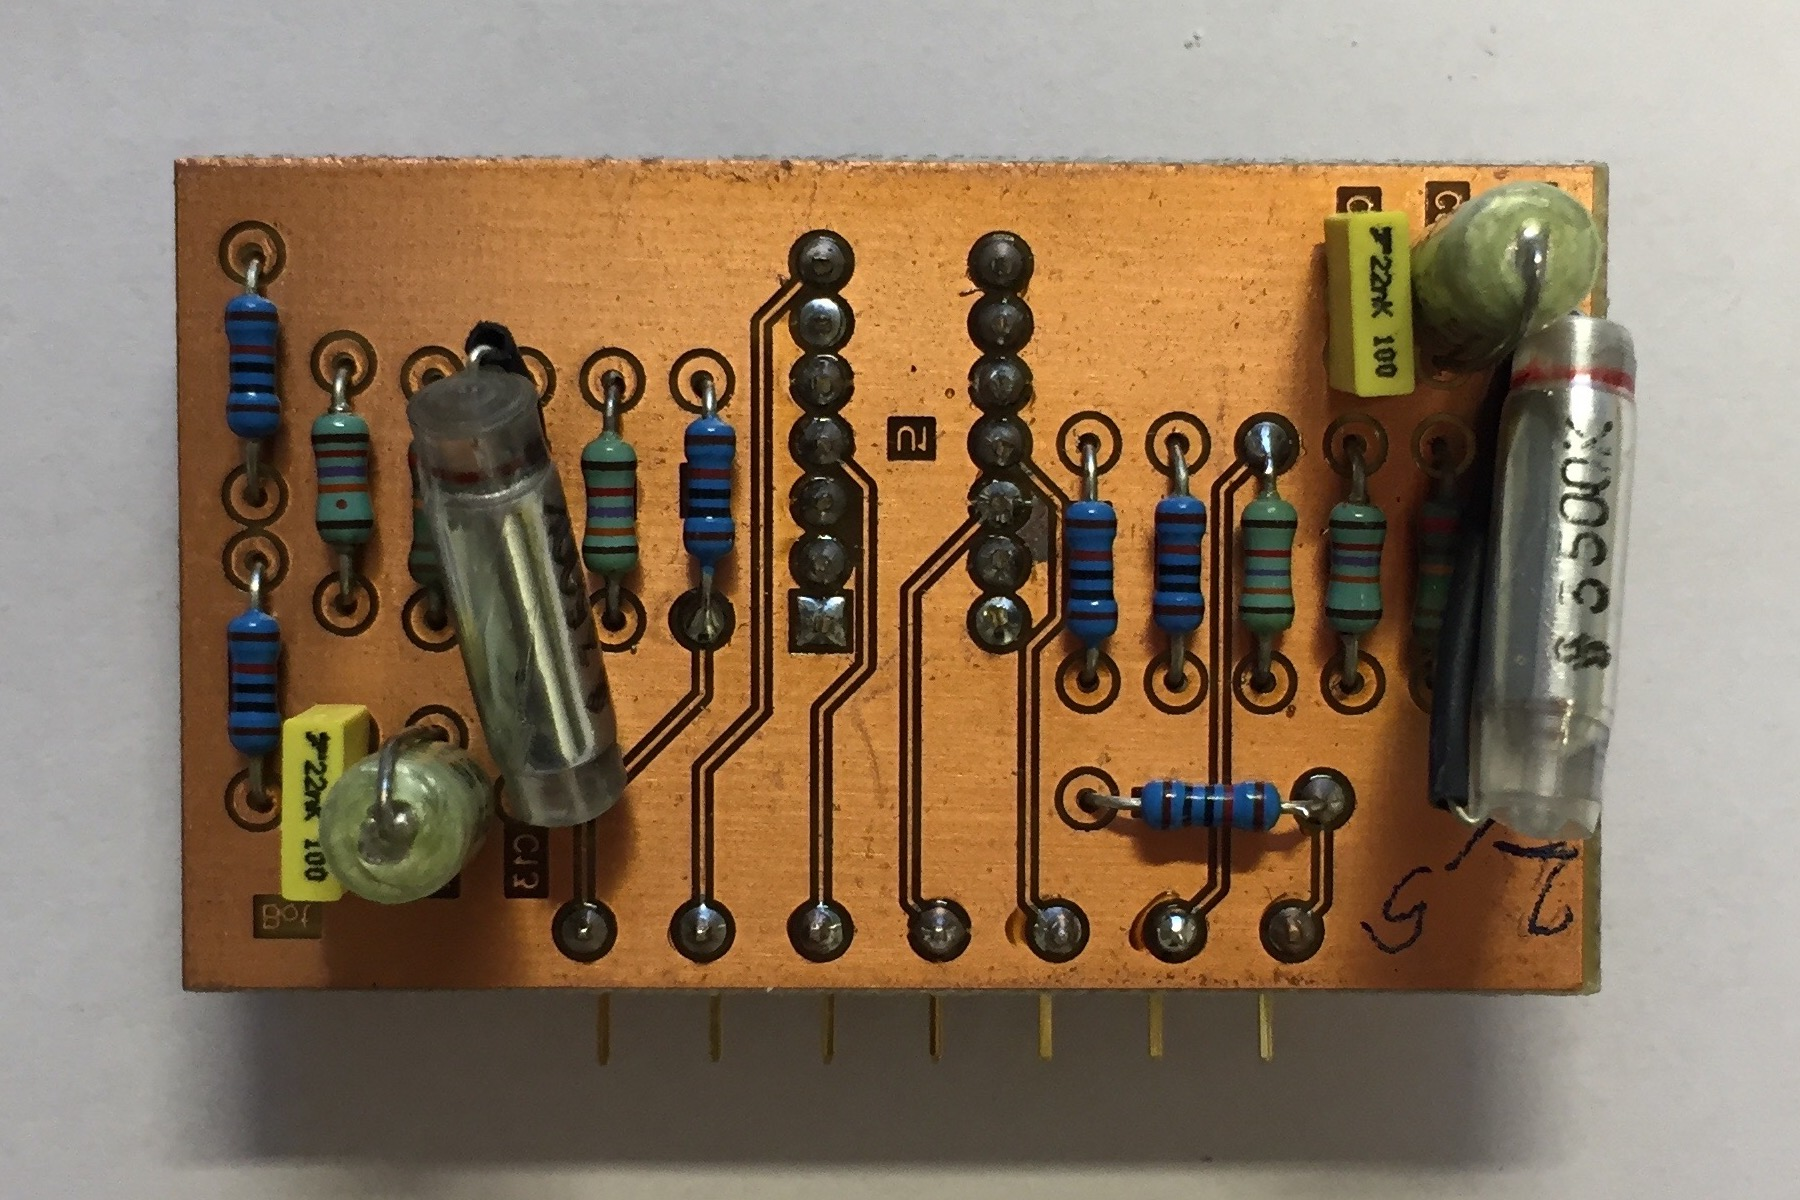
\includegraphics[resolution=300,width=\textwidth/2]{ProductShots/Filter2_5Front}
	\caption{Færdigt filter for $\pm$2.62dB}
	\label{fig:Filter2_5Front}
\end{figure}
\noindent
%
%
\begin{table}[H]
\centering
\begin{tabular}{|c|r|r|r|}
\hline
\multicolumn{1}{|l|}{Komponenter} & \multicolumn{1}{l|}{Beregnet} & \multicolumn{1}{l|}{Brugt} & \multicolumn{1}{l|}{Afvigelse [$\%$]}\\ \hline
$R_i$ & 10k$\Omega$ & 10k$\Omega$ & 0\\ \hline
$R_F$ & 18.281k$\Omega$ & 18.7k$\Omega$ & 2.292 \\ \hline
$R_1$ & 82.074k$\Omega$ & 82.5k$\Omega$ & 0.519 \\ \hline
$R_2$ & 67.123k$\Omega$ & 66.5k$\Omega$ & 0.9281 \\ \hline
$R_3$ & 54.896k$\Omega$ & 54.9k$\Omega$ & 0.0073 \\ \hline
$C_1$ & 28.835nF & 33nF & 14.4443 \\ \hline
$C_2$ & 13.408nF & 15nF & 11.8735 \\ \hline
$C_3$ & 6.235nF & 6.8nF & 9.0617 \\ \hline
\end{tabular}
\caption{Komponentværdier for de filtre der forstærker $\pm$5.24dB.}
\label{tab:TilpasningAfFiltre5.24}
\end{table}
%
\begin{figure}[H]
	\centering
	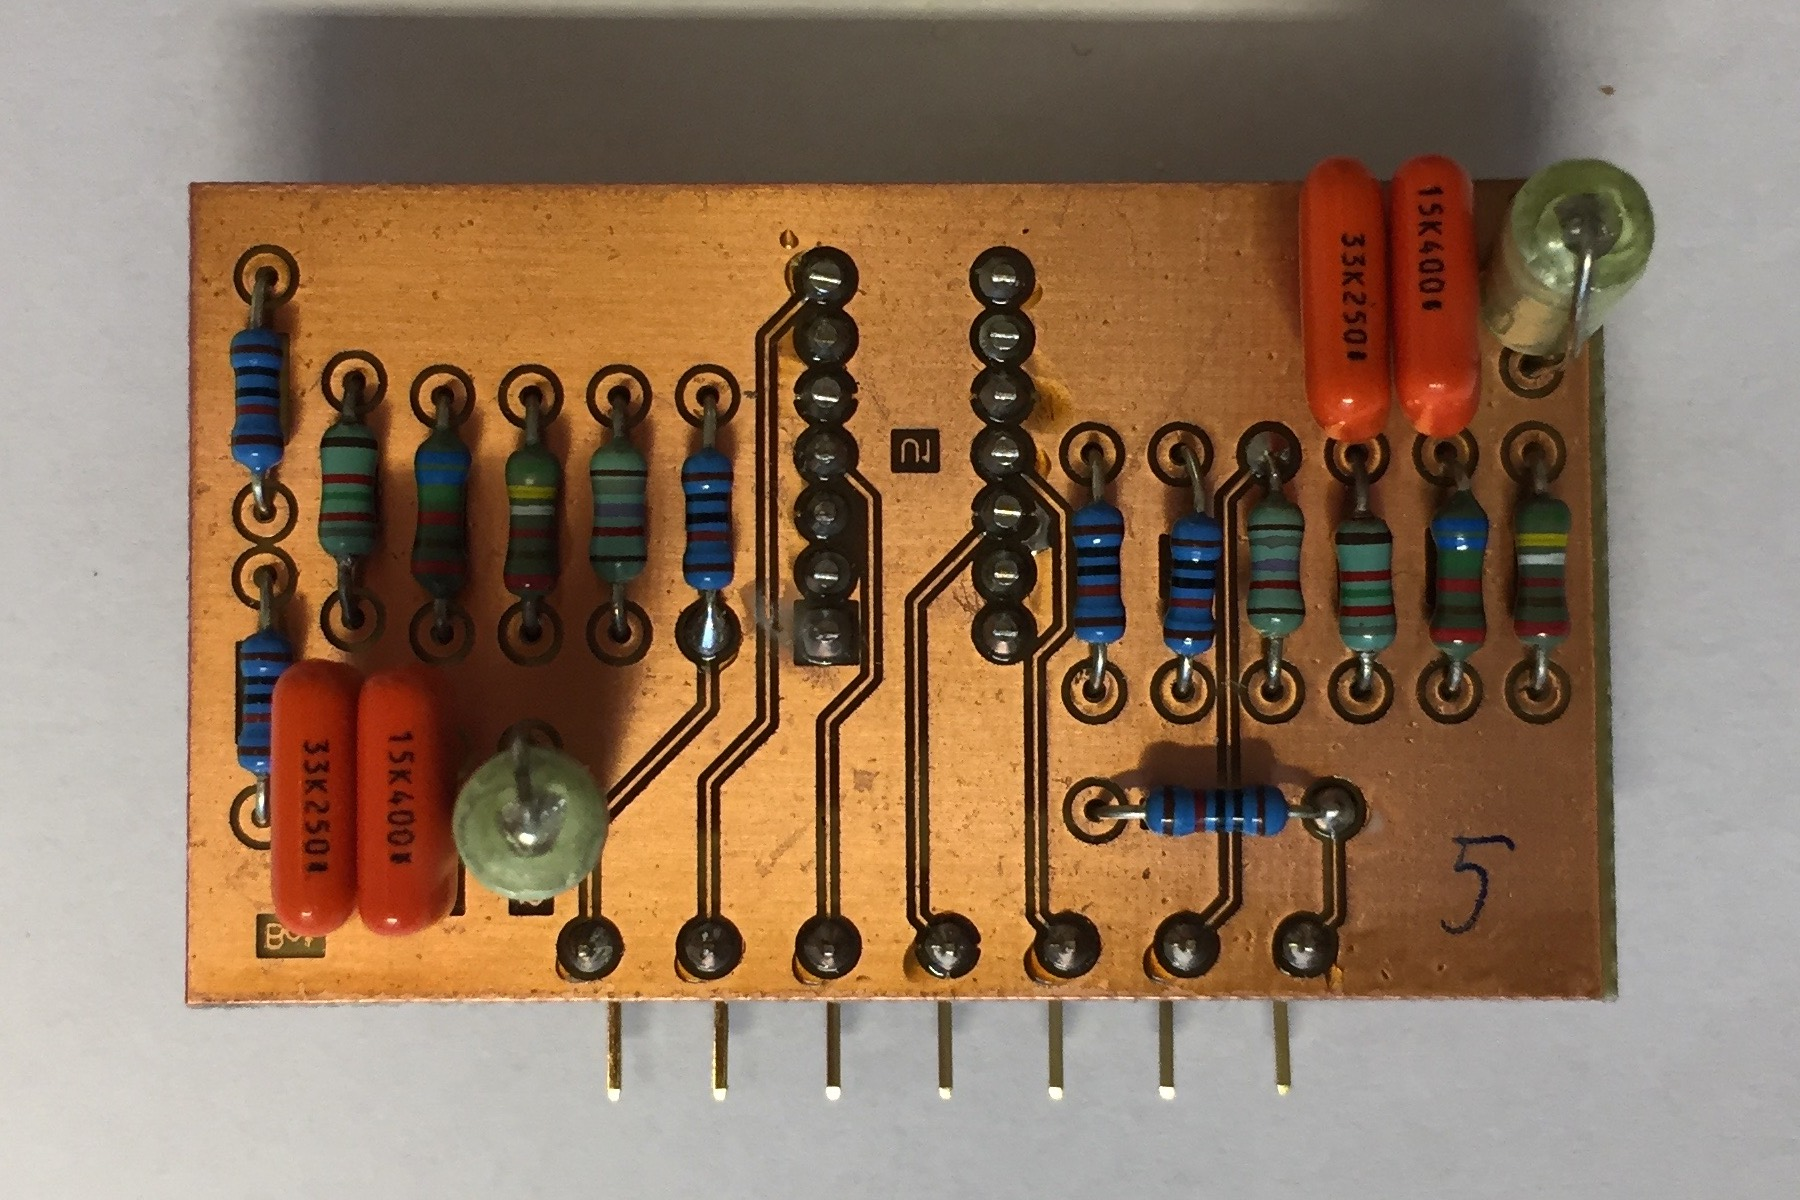
\includegraphics[resolution=300,width=\textwidth/2]{ProductShots/Filter5Front}
	\caption{Færdigt filter for $\pm$5.24dB}
	\label{fig:Filter5Front}
\end{figure}
\noindent
%
%
\begin{table}[H]
\centering
\begin{tabular}{|c|r|r|r|}
\hline
\multicolumn{1}{|l|}{Komponenter} & \multicolumn{1}{l|}{Beregnet} & \multicolumn{1}{l|}{Brugt} & \multicolumn{1}{l|}{Afvigelse [$\%$]}\\ \hline
$R_i$ & 10k$\Omega$ & 10k$\Omega$ & 0\\ \hline
$R_F$ & 33.42k$\Omega$ & 33.2k$\Omega$ & 0.6583 \\ \hline
$R_1$ & 67.502k$\Omega$ & 66.5k$\Omega$ & 1.4844 \\ \hline
$R_2$ & 45.149k$\Omega$ & 45.3k$\Omega$ & 0.3344 \\ \hline
$R_3$ & 30.198k$\Omega$ & 30.1k$\Omega$ & 0.3245 \\ \hline
$C_1$ & 28.673nF & 33nF & 15.0909 \\ \hline
$C_2$ & 16.303nF & 15nF & -7.9924 \\ \hline
$C_3$ & 9.269nF & 10nF & 7.8865 \\ \hline
\end{tabular}
\caption{Komponentværdier for de filtre der forstærker $\pm$10.48dB.}
\label{tab:TilpasningAfFiltre10.48}
\end{table}
%
\begin{figure}[H]
	\centering
	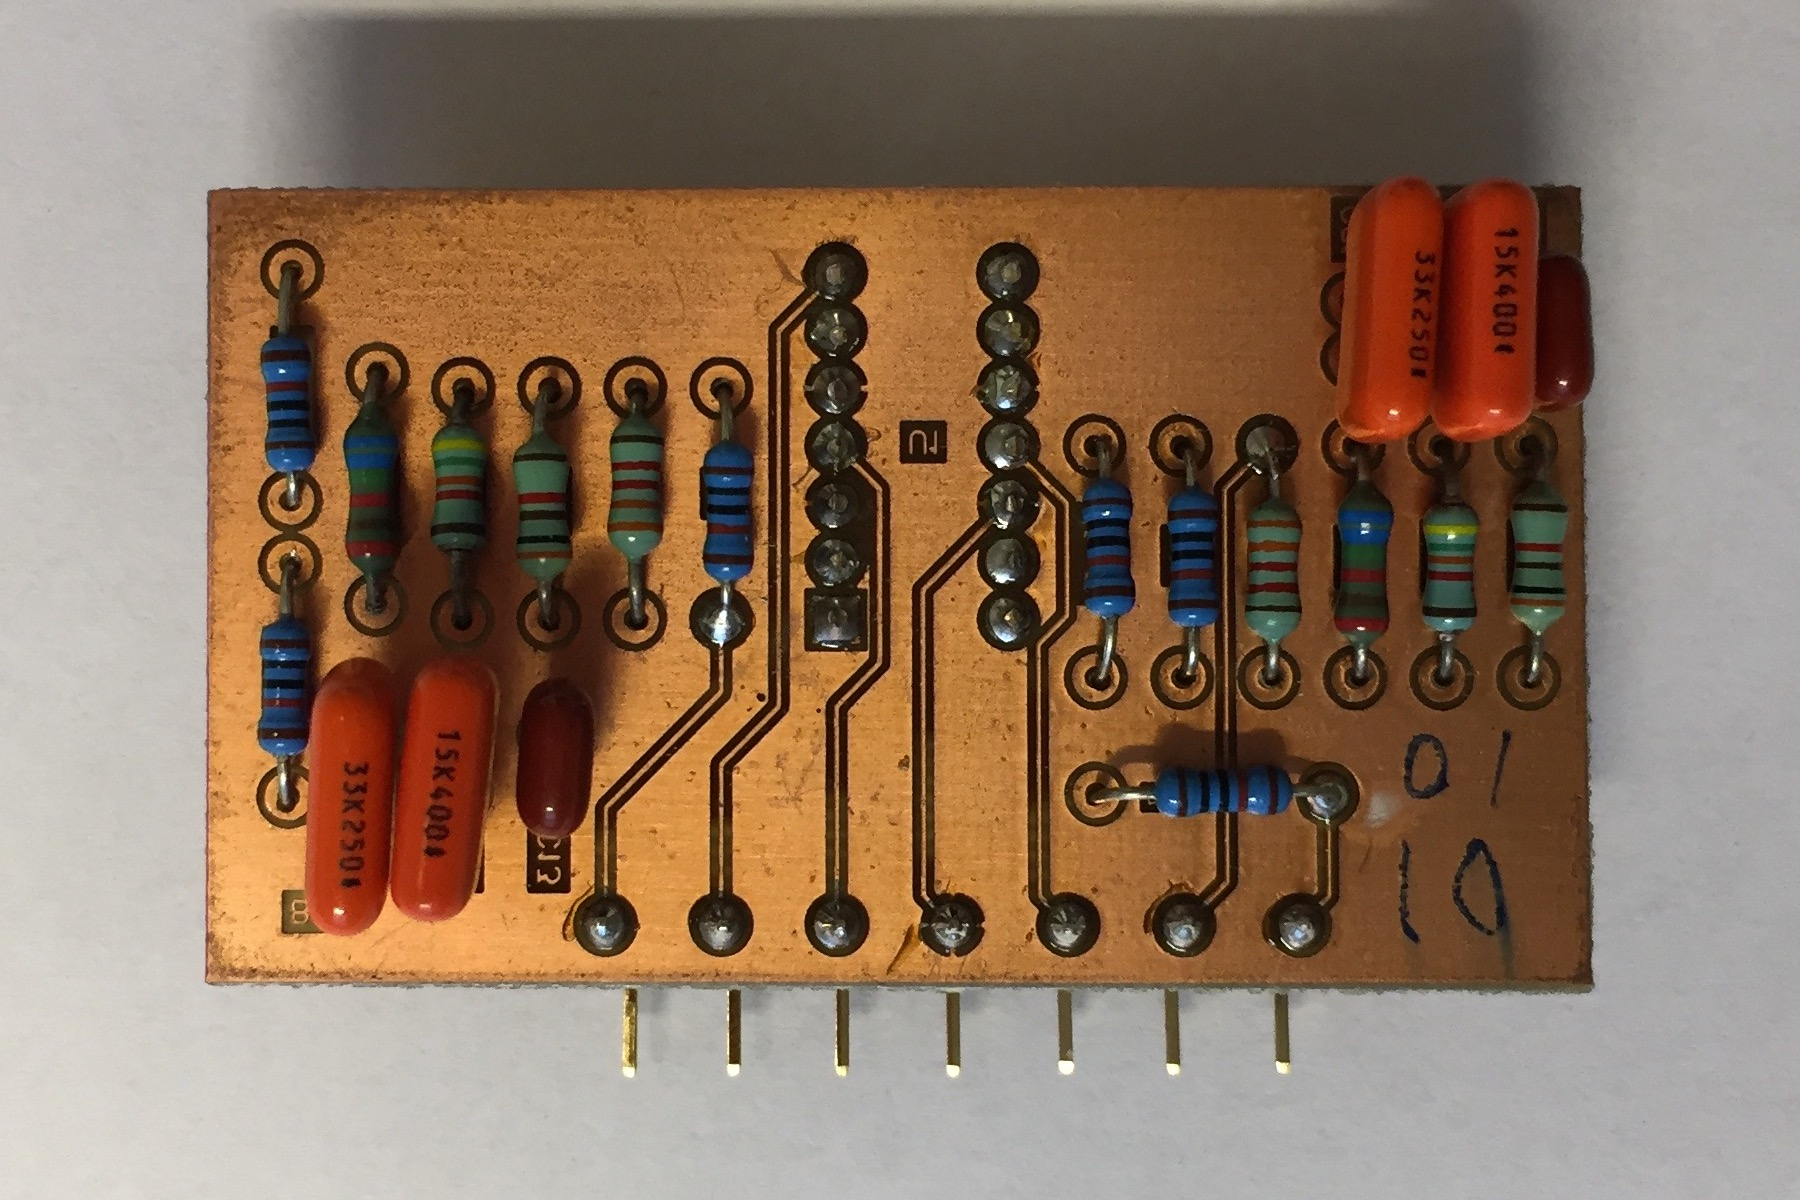
\includegraphics[resolution=300,width=\textwidth/2]{ProductShots/Filter10Front}
	\caption{Færdigt filter for $\pm$10.48dB}
	\label{fig:Filter10Front}
\end{figure}
\noindent
%
%
\begin{table}[H]
\centering
\begin{tabular}{|c|r|r|r|}
\hline
\multicolumn{1}{|l|}{Komponenter} & \multicolumn{1}{l|}{Beregnet} & \multicolumn{1}{l|}{Brugt} & \multicolumn{1}{l|}{Afvigelse [$\%$]}\\ \hline
$R_i$ & 10k$\Omega$ & 10k$\Omega$ & 0\\ \hline
$R_F$ & 111.686k$\Omega$ & 107k$\Omega$ & 4.1957 \\ \hline
$R_1$ & 90.413k$\Omega$ & 88.7k$\Omega$ & 1.8946 \\ \hline
$R_2$ & 40.448k$\Omega$ & 40.2k$\Omega$ & 0.6131 \\ \hline
$R_3$ & 18.095k$\Omega$ & 17.8k$\Omega$ & 1.6303 \\ \hline
$C_1$ & 14.318nF & 15nF & 4.7632 \\ \hline
$C_2$ & 12.172nF & 12.5nF & 2.6947 \\ \hline
$C_3$ & 10.347nF & 10nF & -3.3536 \\ \hline
\end{tabular}
\caption{Komponentværdier for de filtre der forstærker $+$20.96dB.}
\label{tab:TilpasningAfFiltre20.96}
\end{table}
%
\begin{figure}[H]
	\centering
	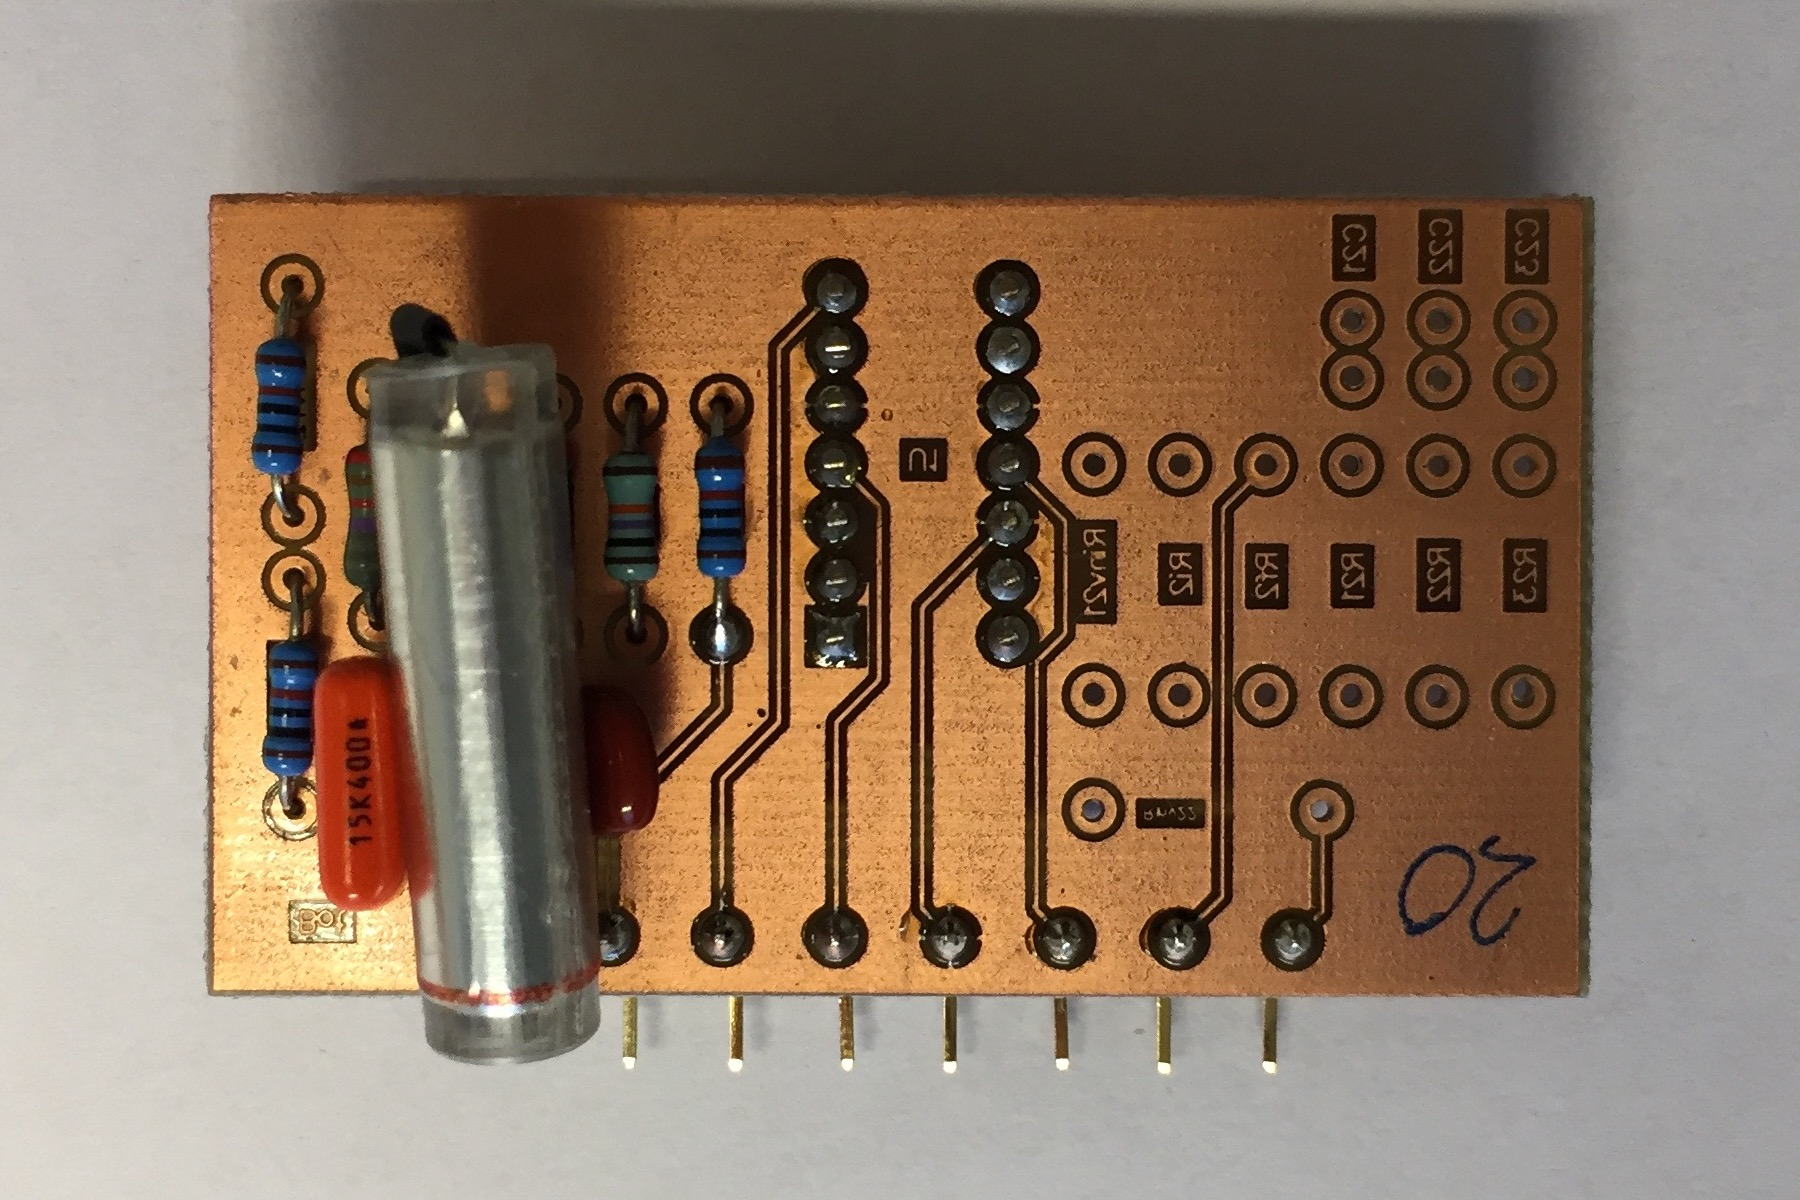
\includegraphics[resolution=300,width=\textwidth/2]{ProductShots/Filter20Front}
	\caption{Færdigt filter for $+$20.96dB}
	\label{fig:Filter20Front}
\end{figure}
%
\newpage
\noindent
%
De beregnede og brugte komponentværdier for de syv filtre, fremsat i \autoref{tab:TilpasningAfFiltre2.62}, \autoref{tab:TilpasningAfFiltre5.24}, \autoref{tab:TilpasningAfFiltre10.48} og \autoref{tab:TilpasningAfFiltre20.96}, afbilledes på \autoref{fig:UdregnetKontraPraktiskGain}.
%
\begin{figure}[H]
	\centering
	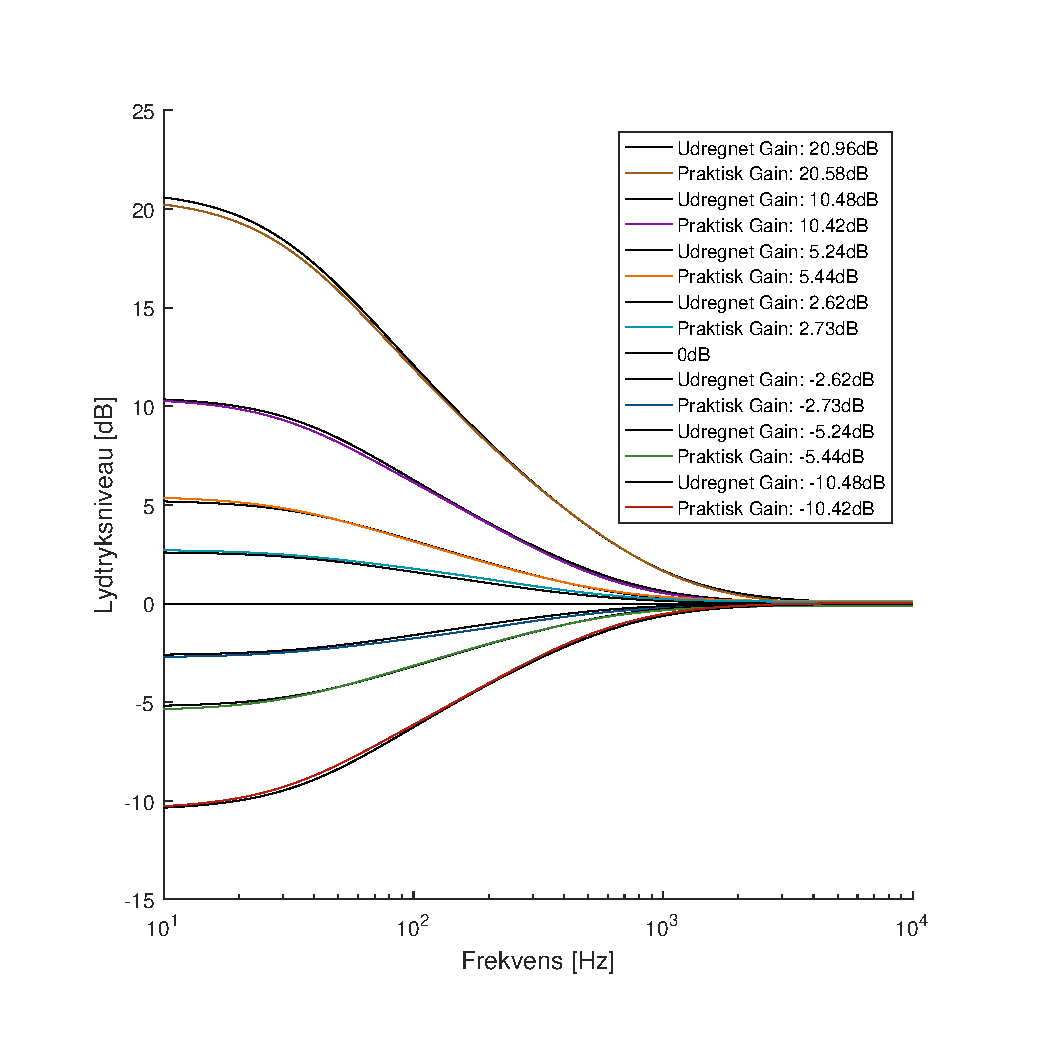
\includegraphics[resolution=300,width=\textwidth]{Figure/DesignAfFilter/UdregnetKontraPraktiskGain.pdf}
	\caption{Kurverne for de beregnede komponentværdier og de brugte komponentværdier sammenholdes. Hvor 0dB angiver én gangs forstærkning.}
	\label{fig:UdregnetKontraPraktiskGain}
\end{figure}
\noindent
%
Ud fra \autoref{fig:UdregnetKontraPraktiskGain} tyder det på, at de afvigelser der måtte være mellem de beregnede og de brugte komponentværdier er af minimal betydning. Data til \autoref{fig:UdregnetKontraPraktiskGain} forefindes i vedlagte mappe, som er navngivet: \textit{SupplerendeMateriale}. 

 



%\subsection{Valg af antal RC-led}
\label{ValgAfAntalRCLed}
2.62dB per 5dB volumen ændring
Vi startet med en figur der viser hældningerne ved 1,2,3,4 RC led, så kan vi komme ``så'' tæt på
så har vi et grundlag for hvorfor et led ikke er nok og hvorfor 4 er for meget
Hvad sker der hvis man har for mange led, hvad kan være negativt ved det? Vi ønsker at holde det simpelt og ``billigt'' 
Hvilke værdier har de forskellige RC-led
Vi fokuserer på 2 og 3 led
Udregninger i bilag, vis et eller to eksempler (for 1 og 2 RC-led) 
Kondensatorerne udvælges efter skøn (bedts muligt fit til kurven)

%Det egentlige afsnit starter her:
Dette afsnit har til formål at finde ud af hvor mange RC-led kredsløbet skal indeholde, svarende til hvor mange brøkdele dæmpningen skal deles op i fra $2.62dB$ til $0dB$.


Der ønskes et maksimalt gain på $2.62dB$, baseret på antagelser lavet i \fullref{ISO226}.
Som udgangspunkt dimensioneres $R_i$ til at være $10K\Omega$.
Gainet på $2.62dB$ omregnes til en gainfaktor:
\begin{equation}
	G_0 = 10^{\frac{2.62}{20}} = 1.3335
\end{equation}
\noindent
Dette er den maksimale forstærkning 



\subsection{1 RC-led}
Når vi regner med et RC-led, skal vi sikre at vi får en forstærkning på 1, svarende til 0dB. 
%
\begin{equation}
	G_1 = 1 = \frac{10K\Omega}{10K\Omega}
\end{equation}
\noindent
%
Så finder vi tilbagekoblingsmodstanden ved $G_1$
%
\begin{equation}
	R_f' = R_i*G_1 = 10K\Omega*1 = 10K\Omega
\end{equation}
\noindent
%
Så kan vi beregne $R_1$
%
\begin{equation}
	R_1 = \frac{R_f*R_f'}{R_f-R_f'} = \frac{13.335K\Omega*10K\Omega}{13.335K\Omega-10K\Omega} = 39.983K\Omega
\end{equation}
\noindent
%indsæt resten af formlerne for 2 og 3 led
Når alle gains er udregnet for 1-8 RC-led kan en kondensatorværdi estimeres ved at udregne værdien hvis man ønsker en knækfrekvens omkring $20 Hz$, dette kan gøres med følgende formel:
\begin{equation}
C_1=\frac{1}{R_1*2*\pi*f}
\end{equation}
Dette er for den første kondensatorværdi og resten kan forsøges at estimere, men da poler og nulpunkter risikerer at overlappe. (hvilket risikerer i stejlere og tidligere hældning)
Derfor kan det være svært at komme regne sig frem til den præcise værdi af $C$, simulering kan derfor være en bedre fremgangsmåde for at fastslå den endelige værdi af alle $C-ledene$. 
Udover at de enkelte poler kan overlappe er den generelt svært at estimere hvilken frekvens den næste pol skal ligge ved, (hvad skal fremgangsmåden være?)
Eftersom der ønskes en lineær hældning vil en lineær hældning for frekvensresponsen bestræbes der også et lineært forløb for afskæringsfrekvensen.

%indsæt udregningerne af logstep og dernæst C
%
\begin{figure}[H]
	\centering
	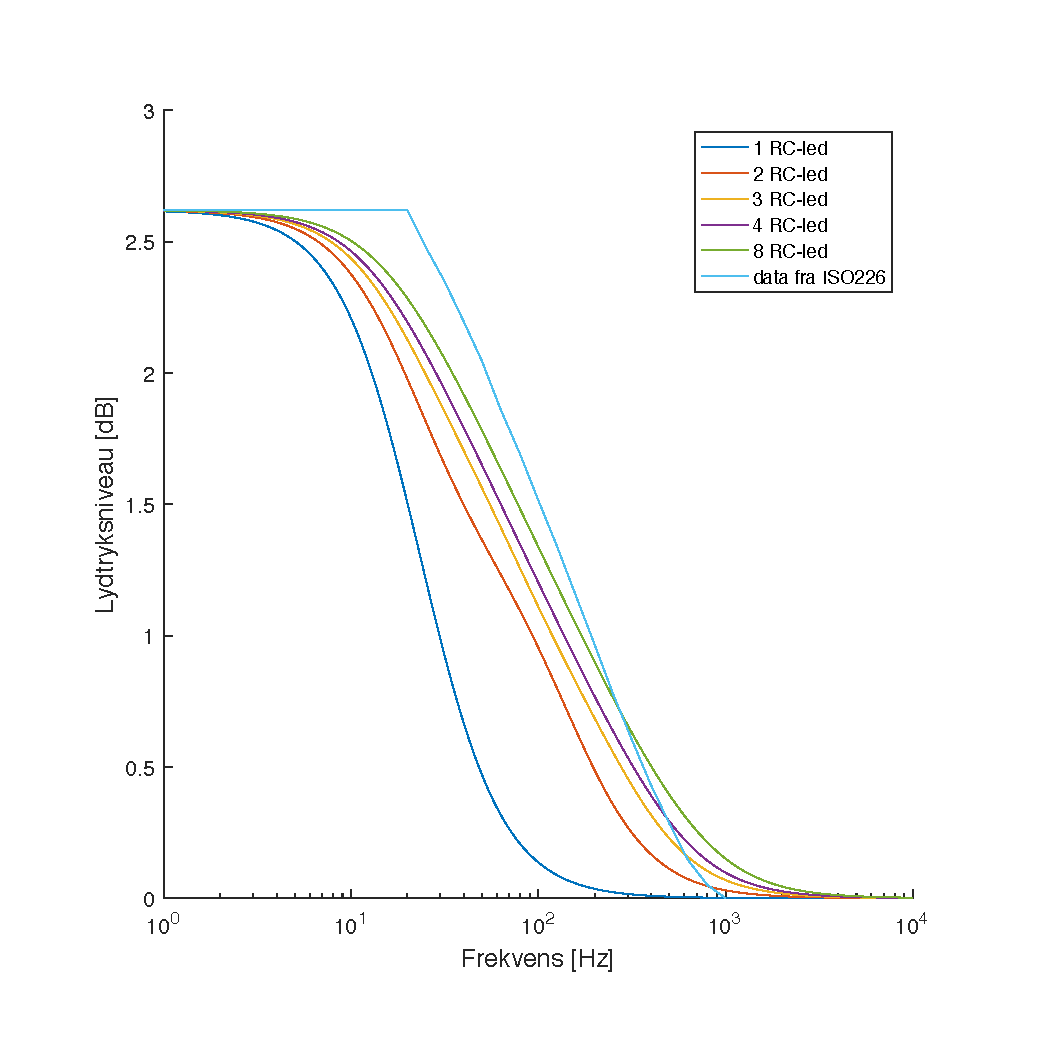
\includegraphics[resolution=300,width=\textwidth]{Figure/DesignAfFilter/1,2,3,4,8RC-ledGain2,62.pdf}
	\caption{Overføringsfunktion for filtre med henholdsvis 1,2,3,4 og 8 RC-led, hvor den logaritmiske x-akse angiver frekvens i hertz og den lineære y-akse angiver lydtryksniveau i dB.}
	\label{fig:1-8RC-ledIkkeJusteretC}
\end{figure}
\noindent
%
På \autoref{fig:1-8RC-ledIkkeJusteretC} illustreres den forskellige overføringsfunktioner for filtrene med et gain på $2.62 dB$ med tilhørende poler udregnet til $20 Hz$.
%Der er lavet flere forskellige plots som hver illustrer effekten af at tilføje flere led til filtret.
Der ønskes som sagt et så lineært forløb, mellem to punkter der henholdsvis har en forstærkning af signalet på $2.62 dB$ ved $20 Hz$ samt en forstærkning på $0 dB$ ved $1000 Hz$.
Filtret med 1 RC-led fravælges da det ikke har den tilsigtede hældning, det har en for stejl hældning.
Denne hældning kan ikke justeres da pol og nulpunkt parret kun kan flyttes ud ad x-aksen.
Filtret med 2 RC-led fravælges da det ikke har et lineært forløb efter indrulningsforløbet, men et mindre knæk opad på grafen omkring XX$1 dB$.
Derimod har filtret med 3 RC-led et meget lineært forløb uden betydelige knæk på grafen, samt en hældning der stemmer overens med det af den ønskede.
Funktionen knækker for tidligt i forhold til det ønskede, dette kompenseres der senere for med justering af hvor den første pol befinder sig.
Filtrene med 4 og 8 RC-led fravælges da det vurderes redundant at indføre unødige led, da de ønskede specifikationer kan opnås med færre komponenter, altså filtret med 3 RC-led.

Med dette vælges det derfor at udføre filtersystemet med et fraktalordensfilter der indeholder 3 RC-led.
Videre finjustering af filtrene med 3 RC-led foretages i \autoref{TilpasningAfFilter}.







%Her illustrerer knækkene tydeligt at afskæringsfrekvensen er for lav og videre justering bliver gjort manuelt i simuleringsprogrammet \textit{LTspice}.

%møde
%hvordan findes de andre C værdier
%Hvordan ved vi hvad der er godt nok
%Pænt nok= ingen krumninger over forløbet
%det er ok at simulere sig frem til C led (sofus har en udregningsmetode til at finde poler og nulpunkter)

%minus 2's kompliment


%pol(knæk nedad)
%nulpunkt(den retter ud)

%find forskrift med kvotienter
%find $r^2$
%\subsection{To RC-led}
\label{ToRCLed}
Når der beskæftiges med realtionen mellem et indgangssignal og et udgangssignal, tænkes der på, hvilken forstærkning eller dæmpning, der sker i systemet. Dette beskrives med overføringsfunktionen, der generelt lyder:
\begin{equation}
	H(S)=\frac{Y(S)}{X(S)}
\quad
	<=>
\quad	
	Y(S)=H(S)*X(S)
\end{equation}

\noindent
$X(S)$ beskriver indgangssignalet, $Y(S)$ beskriver udgangssignalet og $H(S)$ beskriver den pågældende forstærkning eller dæmpning, der ganget med $X(S)$ er produktet af $Y(S)$. Dette er uafhængigt af om der kigges på forstærkning af strøm eller spænding. \\

\noindent
Ved tilføjelsen af et nyt RC-led omregnes $R_F$ og $R_1$ til ét led, $R_F'$. Kondensatoren $C_1$ ses der bort fra i denne sammenhæng, da den ikke påvirker forstærkningen/dæmpningen. Kondensatoren bestemmer i stedet, hvornår de forskellige led ruller ind. Der er derfor blot tale om to modstande, der sidder parallelt, som skal regnes sammen til én modstand. Det foregår på følgende måde: \\

\begin{equation}
	R_F'= \frac{R_F*R_1}{R_F+R_1}
\end{equation}\\

\noindent
Med dette kommer en overføringsfunktion for et filter med 2 RC-led til at hedde:\\

\begin{equation}
	\frac{V_o}{V_i}=-\frac{R_F'||(R_2+\frac{1}{SC_2})}{R_i}
\quad
	<=>
\quad
	\frac{V_o}{V_i}=-\frac{R_F'*(R_2+\frac{1}{SC_2})}{R_i*(R_F'+(R_2+\frac{1}{SC_2}))}
\end{equation}\\

\noindent
Det er herefter muligt at reducere udtrykket ved at reducere antallet af brøkstreger. Eksempelvis kan der ganges $SC_2$ på både over og under brøkstregen, hvilket vil reducere den samlede funktion. Endvidere samles $-\frac{R_F'}{R_i}$ på med sin egen brøkstreg.\\

\begin{equation}
	\frac{V_o}{V_i}=-\frac{R_F'}{R_i}* \frac{R_2*SC_2+1}{R_F'*SC_2+R_2*SC_2+1}
\quad
	<=>
\quad
	\frac{V_o}{V_i}=-\frac{R_F'}{R_i}*\frac{R_2*SC_2+1}{SC_2(R_F'+R_2)+1}\\
\end{equation}\\

\noindent
Poler og nulpunkter

\begin{equation}
	\frac{V_o}{V_i}=-\frac{R_F'}{R_i}*\frac{\frac{S}{\omega Z}+1}{\frac{S}{\omega P}+1}
\end{equation}
%\subsection{Tre RC-led}
\label{TreRCLed}

Matematisk er fremgangsmåden den samme, når der sættes flere RC-led på. Ved tilføjelsen af et tredje RC-led er der blot tale om 3 modstande i parallelforbindelse, der skal omregnes til én korresponderende modstand, der med 3 led kommer til at hedde $R_F''$:

\begin{equation}
	R_F''=R_F||R_1||R_2
\end{equation}

\noindent
Herefter er fremgangsmåden for at finde frem til en overføringsfunktion for systemet den samme. Det er vigtigt først at tage højde for antallet af RC-led. Herefter ligner udregningerne hinanden, uafhængigt af om der er 2, 3 eller flere RC-led:\\

\begin{equation}
	\frac{V_o}{V_i}=-\frac{R_F''||(R_2+\frac{1}{SC_2})}{R_i}
\quad
	<=>
\quad
	\frac{V_o}{V_i}=-\frac{R_F''*(R_2+\frac{1}{SC_2})}{R_i*(R_F''+(R_2+\frac{1}{SC_2}))}
\end{equation}\\


\begin{equation}
		\frac{V_o}{V_i}=-\frac{R_F''}{R_i}* \frac{R_2*SC_2+1}{R_F''*SC_2+R_2*SC_2+1}
\quad
	<=>
\quad
	\frac{V_o}{V_i}=-\frac{R_F''}{R_i}*\frac{R_2*SC_2+1}{SC_2(R_F''+R_2)+1}
\end{equation}\\


\noindent
Poler og nulpunkter

\begin{equation}
	\frac{V_o}{V_i}=-\frac{R_F'}{R_i}*\frac{\frac{S}{\omega Z}+1}{\frac{S}{\omega P}+1}
\end{equation}


